\chapter{The Map: Two Directions of Probability and the Pipeline from Data to Physics}\label{ch:00}
\providecommand{\zeroaEx}[1]{\refstepcounter{wex}\paragraph*{Example~\thewex\ (#1).}}
\providecommand{\CoinPkFair}{}\renewcommand{\CoinPkFair}{0.04395}
\providecommand{\CoinPkBias}{}\renewcommand{\CoinPkBias}{0.302}
\providecommand{\CoinSimFair}{}\renewcommand{\CoinSimFair}{0.04105}
\providecommand{\CoinSimBias}{}\renewcommand{\CoinSimBias}{0.3024}
\providecommand{\CoinSimErr}{}\renewcommand{\CoinSimErr}{0.001449}
\providecommand{\CoinPostBias}{}\renewcommand{\CoinPostBias}{0.873}
\providecommand{\CoinPostBiasFive}{}\renewcommand{\CoinPostBiasFive}{0.09696}
\providecommand{\CoinLR}{}\renewcommand{\CoinLR}{6.872}
\providecommand{\CoinNexp}{}\renewcommand{\CoinNexp}{20000}
\providecommand{\QSdTen}{}\renewcommand{\QSdTen}{0.1267}
\providecommand{\QSdHundred}{}\renewcommand{\QSdHundred}{0.03997}
\providecommand{\QSdTenTh}{}\renewcommand{\QSdTenTh}{0.1265}
\providecommand{\QSdHundredTh}{}\renewcommand{\QSdHundredTh}{0.04}
\providecommand{\QMeanTen}{}\renewcommand{\QMeanTen}{0.7993}
\providecommand{\QPexact}{}\renewcommand{\QPexact}{0.05469}
\providecommand{\QPmcMillion}{}\renewcommand{\QPmcMillion}{0.0545}
\providecommand{\QSigmaMillion}{}\renewcommand{\QSigmaMillion}{2.274\times10^{-4}}
\providecommand{\QPmcHundred}{}\renewcommand{\QPmcHundred}{0.0566}
\providecommand{\QNhundred}{}\renewcommand{\QNhundred}{106}
\providecommand{\PipeMaxDiff}{}\renewcommand{\PipeMaxDiff}{3.469\times10^{-18}}
\providecommand{\PipeKTen}{}\renewcommand{\PipeKTen}{7}
\providecommand{\PipeSdTen}{}\renewcommand{\PipeSdTen}{0.1307}
\providecommand{\PipeSdThTen}{}\renewcommand{\PipeSdThTen}{0.1449}
\providecommand{\PipeKHundred}{}\renewcommand{\PipeKHundred}{76}
\providecommand{\PipeSdHundred}{}\renewcommand{\PipeSdHundred}{0.04238}
\providecommand{\PipeSdThHundred}{}\renewcommand{\PipeSdThHundred}{0.04271}
\providecommand{\PipeKThousand}{}\renewcommand{\PipeKThousand}{819}
\providecommand{\PipeSdThousand}{}\renewcommand{\PipeSdThousand}{0.01217}
\providecommand{\PipeSdThThousand}{}\renewcommand{\PipeSdThThousand}{0.01218}
\providecommand{\PipeSdExactTen}{}\renewcommand{\PipeSdExactTen}{0.131}
\providecommand{\SameVarA}{}\renewcommand{\SameVarA}{1}
\providecommand{\SameVarB}{}\renewcommand{\SameVarB}{1}
\providecommand{\SamePkMaxDev}{}\renewcommand{\SamePkMaxDev}{1.500\times10^{-12}}
\providecommand{\SameSkewA}{}\renewcommand{\SameSkewA}{2.455}
\providecommand{\SameSkewB}{}\renewcommand{\SameSkewB}{0.02076}
\providecommand{\SameBzeroA}{}\renewcommand{\SameBzeroA}{51}
\providecommand{\SameBzeroB}{}\renewcommand{\SameBzeroB}{3}
\providecommand{\SameBzeroAzero}{}\renewcommand{\SameBzeroAzero}{34}
\providecommand{\SameBzeroBzero}{}\renewcommand{\SameBzeroBzero}{19}
\providecommand{\SameMinA}{}\renewcommand{\SameMinA}{-0.5344}
\providecommand{\SameNblob}{}\renewcommand{\SameNblob}{60}
\providecommand{\ColMuHat}{}\renewcommand{\ColMuHat}{0.959}
\providecommand{\ColMuLo}{}\renewcommand{\ColMuLo}{0.805}
\providecommand{\ColMuHi}{}\renewcommand{\ColMuHi}{1.116}
\providecommand{\ColNtot}{}\renewcommand{\ColNtot}{4769}
\providecommand{\CmbMeanRatio}{}\renewcommand{\CmbMeanRatio}{1.002}
\providecommand{\CmbScatterLow}{}\renewcommand{\CmbScatterLow}{0.2324}
\providecommand{\CmbScatterHigh}{}\renewcommand{\CmbScatterHigh}{0.02923}
\providecommand{\GwMeanRatio}{}\renewcommand{\GwMeanRatio}{1.006}
\providecommand{\GwNbins}{}\renewcommand{\GwNbins}{8192}
\providecommand{\SeedIdentical}{}\renewcommand{\SeedIdentical}{yes}
\providecommand{\SeedFirstDraw}{}\renewcommand{\SeedFirstDraw}{0.217}
\providecommand{\SeedOtherFirstDraw}{}\renewcommand{\SeedOtherFirstDraw}{0.4034}
\providecommand{\PiHat}{}\renewcommand{\PiHat}{3.143}
\providecommand{\PiErr}{}\renewcommand{\PiErr}{0.001641}
\providecommand{\PiN}{}\renewcommand{\PiN}{1000000}
\section*{Where this chapter is going}
\addcontentsline{toc}{section}{Where this chapter is going}

Two ideas fix the questions that every later chapter answers. The first is
that probability runs in two directions. Forward, it goes from a hypothesis to
the outcomes that hypothesis can produce. Backward, it goes from an outcome
that has already happened to the hypotheses that could have produced it.
Bayes' theorem connects the two directions. The second idea is that a
physicist never feeds raw data straight into Bayes' theorem. First we decide
which information in the data matters. Then we compress the data into a
summary. Then we work out how that summary fluctuates from one experiment to
the next. These steps form one pipeline, from a physical model to a statement
about physics, and the whole book is organised along it. Very little is proved
and only small things are computed; the aim is to see the questions clearly.
The practical side comes last: how the Python code for every chapter is laid
out and how to run it.

\begin{figure}[htbp]
\centering
\begin{tikzpicture}[
  stage/.style={draw=accent,thick,rounded corners=2pt,fill=ideabg,align=center,
                font=\small,text width=3.3cm,minimum height=1.25cm},
  flow/.style={->,thick,accent}]
  \node[stage] (s1) at (0,0)    {\S\ref{0a:sec:two-directions}\\ two directions:\\ prediction, inference};
  \node[stage] (s2) at (4.2,0)  {\S\ref{0a:sec:questions}\\ the questions and\\ the tools that answer them};
  \node[stage] (s3) at (8.4,0)  {\S\ref{0a:sec:pipeline}\\ the pipeline\\ model $\to$ data $\to$ physics};
  \node[stage] (s4) at (8.4,-2.2) {\S\ref{0a:sec:summaries}\\ which summary?\\ amplitude \dots\ topology};
  \node[stage] (s5) at (4.2,-2.2) {\S\ref{0a:sec:universal}\\ same idea, three\\ detectors};
  \node[stage] (s6) at (0,-2.2) {\S\ref{0a:sec:code}\\ running\\ the code};
  \draw[flow] (s1) -- (s2);
  \draw[flow] (s2) -- (s3);
  \draw[flow] (s3) -- (s4);
  \draw[flow] (s4) -- (s5);
  \draw[flow] (s5) -- (s6);
\end{tikzpicture}
\caption{The route through the ideas. The top row sets up the logic: the
two directions of probability, the list of questions they generate, and the
pipeline that strings the questions together. The bottom row makes it
concrete: what we choose to measure from a field, how the same logic looks in
three different experiments, and how to reproduce every number in the book.}
\label{0a:fig:roadmap}
\end{figure}

\section{Two directions of probability}\label{0a:sec:two-directions}

A friend runs a magic shop. In one drawer she keeps coins of two kinds, mixed
together in equal numbers: honest coins, and trick coins weighted so that they
land heads 80\% of the time. The two kinds look identical. She takes one coin
out at random and we toss it ten times. It lands heads 8 times.

Two different questions can be asked about this coin, and they must not be
confused. The first could be asked \emph{before} the tosses: ``if this coin is
honest, how likely is it to give 8 heads in 10 tosses?'' The second is the one
we actually want \emph{after} the tosses: ``we have seen 8 heads; which kind of
coin is it, and how sure can we be?'' Each question asks for a conditional
probability, and Bayes' theorem turns an answer to the first into an answer to
the second. Every later calculation in the book, from a $p$-value to an MCMC
chain over six cosmological parameters, answers one of these two questions.

\paragraph{Forward and inverse problems.}
Physics already knows this distinction. Given a Hamiltonian and an initial
state, working out where the particle goes is the \emph{forward} problem, and
it has one answer. Given the hits in a tracking detector, working out which
track, momentum and vertex produced them is the \emph{inverse} problem.
Several tracks could have produced similar hits, so we must weigh them against
each other. Probability in the forward direction is like integrating the
equations of motion. Probability in the backward direction, called inference,
is like track reconstruction: we hold the outcome and reason back to its cause.

\paragraph{Prediction versus inference.}
Probability answers two kinds of question.
\begin{center}
\small
\begin{tabular}{@{}p{0.44\linewidth}p{0.44\linewidth}@{}}
\toprule
\textbf{Prediction} & \textbf{Inference}\\
\midrule
Start with a hypothesis $H$. & Start with an observed event $E$.\\
Ask what outcomes it can produce, and how often. & Ask which hypotheses might lie behind it, and how probable each is now.\\
Use $\Prob(E\given H)$. & Want $\Prob(H\given E)$.\\
Forward direction: $H\to E$. & Reverse direction: $E\to H$.\\
\bottomrule
\end{tabular}
\end{center}
These are not two rival interpretations of probability. They are two
different questions asked of the same probabilities: the probabilities of
every combination of hypothesis and outcome.

In the backward direction, ask two questions in words before writing any
symbol. Which hypotheses could have produced what we saw? How probable was
what we saw under each of them? \Cref{ch:05} makes this a working habit.

A \newterm{probability tree} shows both directions at once. The first set of
branches chooses the hypothesis (which coin). The second set chooses the
outcome (8 heads or not). Each branch carries the probability of taking it,
\emph{given that we have reached the node it leaves from}. Multiplying the
numbers along a path gives the probability of the whole path.

\begin{figure}[htbp]
\centering
\begin{tikzpicture}[
  nd/.style={font=\small,align=center},
  br/.style={thick,softgray},
  obs/.style={very thick,bdryred}]
  \node[nd,draw,rounded corners=2pt] (root) at (0,0) {drawer};
  \node[nd] (F) at (3.6,1.5)  {fair, $p=\tfrac12$};
  \node[nd] (B) at (3.6,-1.5) {biased, $p=0.8$};
  \node[nd,font=\scriptsize,softgray] at (3.6,1.05)  {$\Prob(F)=\tfrac12$};
  \node[nd,font=\scriptsize,softgray] at (3.6,-1.95) {$\Prob(B)=\tfrac12$};
  \node[nd,bdryred] (F8) at (8.2,2.1)  {8 heads};
  \node[nd,softgray] (Fn) at (8.2,0.9) {not 8 heads};
  \node[nd,bdryred] (B8) at (8.2,-0.9) {8 heads};
  \node[nd,softgray] (Bn) at (8.2,-2.1) {not 8 heads};
  \draw[br] (root.east) -- (F.west);
  \draw[br] (root.east) -- (B.west);
  \draw[obs] (F.east) -- (F8.west);
  \draw[br] (F.east) -- (Fn.west);
  \draw[obs] (B.east) -- (B8.west);
  \draw[br] (B.east) -- (Bn.west);
  \node[nd,font=\scriptsize,anchor=west] at (F8.east) {$\Prob(8\given F)=0.0439$};
  \node[nd,font=\scriptsize,anchor=west,softgray] at (Fn.east) {$0.9561$};
  \node[nd,font=\scriptsize,anchor=west] at (B8.east) {$\Prob(8\given B)=0.302$};
  \node[nd,font=\scriptsize,anchor=west,softgray] at (Bn.east) {$0.698$};
\end{tikzpicture}
\caption{The coin as a probability tree. Read left to right, it is a
prediction machine: pick a coin, then see what that coin tends to produce.
Inference reads it the other way. We have observed ``8 heads'', so only the
two red paths survive; the question is how the total probability of those two
paths is split between the fair coin and the biased one.}
\label{0a:fig:coin-tree}
\end{figure}

\paragraph{The backward direction in four steps.}
Before any equation, put the question into words: (1) what did we see?
(2) which hypotheses could have produced it? (3) how probable was it under each
of them? (4) how must the probabilities the hypotheses had beforehand change in
view of it?

\emph{The event.} What we observed is ``8 heads in 10 tosses''.

\emph{What could have produced it?} The one thing we do not know is which kind
of coin came out of the drawer. So there are two candidate explanations: the
coin is fair ($F$), or the coin is biased ($B$).

\emph{How probable was the event under each?} This is a forward calculation,
done once per candidate: if the coin is fair, how often do ten tosses give 8
heads? If it is biased, how often? These two numbers are written
$\Prob(8\given F)$ and $\Prob(8\given B)$, and \cref{0a:ex:forward} computes them.

\emph{Only then the update.} Weight each path of the tree by the prior
probability of its coin, keep only the paths that end at ``8 heads'', and
rescale so that the surviving weights add up to one.

Step 3 is where conditional probability enters. For each hypothesis it gives
the probability that the event we actually saw would have had, if that
hypothesis were the one nature chose. To write that in symbols we need its
definition.

\begin{workdef}[conditional probability]
For two events $A$ and $B$ \unpack{sets of possible outcomes, e.g.\ $A$ = ``the
coin is biased'', $B$ = ``8 heads''} with $\Prob(A)>0$, the
\newterm{conditional probability} of $B$ given $A$ is
\begin{equation}
  \Prob(B\given A)\defeq\frac{\Prob(A\cap B)}{\Prob(A)} .
  \label{0a:eq:condprob}
\end{equation}
\emph{Operational meaning:} throw away every outcome outside $A$, and measure
the fraction of what is left that also lies in $B$. $A$ becomes the new
reference space \unpack{the ``whole world'' against which fractions are now
measured}. The \newterm{prediction} question is a number $\Prob(E\given H)$
\unpack{fraction of the $H$-world in which $E$ happens}. The
\newterm{inference} question is a number $\Prob(H\given E)$ \unpack{fraction
of the $E$-world in which $H$ was true}.
\end{workdef}

The same overlap $A\cap B$ can be divided by $\Prob(A)$ or by $\Prob(B)$.
Multiply \eqref{0a:eq:condprob} through by its denominator; doing this with
$A$ and $B$ in both orders gives the \newterm{product rule}
\begin{equation}
  \Prob(A\cap B)=\Prob(B\given A)\,\Prob(A)=\Prob(A\given B)\,\Prob(B) .
  \label{0a:eq:product}
\end{equation}
This one line already contains both directions. Think of probability as area.
$\Prob(A\cap B)$ is the area of the overlap. The two conditional probabilities
divide that \emph{same} overlap by two \emph{different} areas, $\Prob(A)$ or
$\Prob(B)$. \Cref{pre:fig:shrink} draws this for the coin.

Now we turn the direction round, from the observed event back to the
hypotheses. Let $H_1,\dots,H_M$ be hypotheses that are
\newterm{mutually exclusive and exhaustive} \unpack{exactly one of them is
true}; for the coin, $M=2$, with $H_1=F$ and $H_2=B$. Let $E$ be the observed
event, here ``8 heads''.
\begin{align}
  \Prob(H_j\given E)
  &\eqby{1} \frac{\Prob(H_j\cap E)}{\Prob(E)} \nonumber\\
  &\eqby{2} \frac{\Prob(E\given H_j)\,\Prob(H_j)}{\Prob(E)} \nonumber\\
  &\eqby{3} \frac{\Prob(E\given H_j)\,\Prob(H_j)}{\sum_{i=1}^{M}\Prob(E\cap H_i)} \nonumber\\
  &\eqby{4} \frac{\Prob(E\given H_j)\,\Prob(H_j)}{\sum_{i=1}^{M}\Prob(E\given H_i)\,\Prob(H_i)} .
  \label{0a:eq:bayes}
\end{align}
\begin{explain}
  \item Definition \eqref{0a:eq:condprob}, with $E$ as the reference space.
  \item Product rule \eqref{0a:eq:product}, used in the other order:
        $\Prob(H_j\cap E)=\Prob(E\given H_j)\Prob(H_j)$.
  \item The pieces $E\cap H_1,\dots,E\cap H_M$ do not overlap (the $H_i$
        exclude each other) and together make up all of $E$ (one $H_i$ is
        always true). Probabilities of non-overlapping pieces add.
  \item Product rule again, inside each term of the sum.
\end{explain}
This is \newterm{Bayes' theorem}. In words,
$\Prob(H_j\given E)\propto\Prob(E\given H_j)\Prob(H_j)$: \emph{take each
hypothesis's prior weight, multiply it by how readily that hypothesis produces
what we saw, and normalise.} The denominator,
$\Prob(E)=\sum_i\Prob(E\given H_i)\Prob(H_i)$, is the \newterm{law of total
probability}. It is the total weight of all the paths in the tree that end at
the observation. The three ingredients have names. $\Prob(H)$ is the
\newterm{prior}: the probability of $H$ before the observation.
$\Prob(E\given H)$, read as a function of the hypothesis $H$ with $E$ held
fixed, is the \newterm{likelihood}. $\Prob(H\given E)$ is the
\newterm{posterior}: the probability of $H$ after the observation.
\Cref{ch:05} develops all of this in full.

\zeroaEx{the forward direction: what does each coin produce?}
\label{0a:ex:forward}
The question is step 3 of the four: if the coin is fair, how probable are 8
heads in 10 tosses, and if it is biased, how probable? Both answers come from
one formula. For a coin with heads probability $p$, tossed $n$ times
independently, the probability of exactly $k$ heads is
\begin{align*}
  \Prob(k\given p)
  &\eqby{1} \sum_{\text{sequences with $k$ heads}} p^{k}(1-p)^{n-k}
   \eqby{2} \binom{n}{k}\,p^{k}(1-p)^{n-k} .
\end{align*}
\begin{explain}
  \item Independent tosses multiply, so one particular sequence with $k$ heads
        and $n-k$ tails has probability $p^k(1-p)^{n-k}$, whatever the order.
        Different sequences are different outcomes, so their probabilities add.
  \item The number of sequences with $k$ heads among $n$ places is the number
        of ways of choosing which $k$ places are heads,
        $\binom nk=\frac{n!}{k!\,(n-k)!}$.
\end{explain}
For our two coins, the fair one with $p=\frac12$ and the biased one with
$p=0.8$, put $n=10$ and $k=8$. Then $\binom{10}{8}=\frac{10\cdot 9}{2}=45$, so
\begin{align*}
  \Prob(8\given F) &\eqby{1} 45\left(\tfrac12\right)^{10} = \frac{45}{1024} = 0.04395,\\
  \Prob(8\given B) &\eqby{2} 45\,(0.8)^{8}(0.2)^{2}=45\times0.16777\times0.04 = 0.3020 .
\end{align*}
\begin{explain}
  \item With $p=\frac12$ every sequence has the same probability $2^{-10}$.
  \item $0.8^8=0.16777$ and $0.2^2=0.04$.
\end{explain}
The biased coin produces ``8 heads'' in about 30\% of its ten-toss runs; the
fair coin in about 4\%.

\zeroaEx{the backward direction: which coin was it?}
\label{0a:ex:backward}
The question is step 4: having seen 8 heads, how probable is it that the coin
is the biased one? We have everything Bayes' theorem \eqref{0a:eq:bayes}
needs. The two hypotheses are $F$ (fair) and $B$ (biased). The drawer held
equal numbers of each, so the priors are $\Prob(F)=\Prob(B)=\frac12$. The
likelihoods are the two forward numbers of \cref{0a:ex:forward}. Then
\begin{align*}
  \Prob(B\given 8)
  &\eqby{1} \frac{\Prob(8\given B)\Prob(B)}{\Prob(8\given B)\Prob(B)+\Prob(8\given F)\Prob(F)}\\
  &\eqby{2} \frac{0.3020}{0.3020+0.04395}
   = \frac{0.3020}{0.3459} = 0.873 .
\end{align*}
\begin{explain}
  \item Bayes' theorem \eqref{0a:eq:bayes}: numerator is the red path through
        $B$ in \cref{0a:fig:coin-tree}, denominator is both red paths.
  \item The common factor $\Prob(B)=\Prob(F)=\frac12$ cancels between numerator
        and denominator.
\end{explain}
So $\Prob(B\given 8)=0.873$ and $\Prob(F\given 8)=0.127$. The coin itself did
\emph{not} change. What changed is how we share probability between the two
coins it could be.

\begin{keyidea}[Bayes' theorem as information shrinking the sample space]
Before the evidence, the whole sample space is relevant. The evidence $E$
tells us that we are somewhere in the region where $E$ is true, so the sample
space \emph{shrinks} to that region. The posterior $\Prob(H\given E)$ is the
fraction of the shrunken region occupied by $H$:
\[
  \Prob(H\given E)=\frac{\text{area of }(H\cap E)}
  {\text{area of }(H\cap E)+\text{area of }(\neg H\cap E)}
  =\frac{\Prob(E\given H)\Prob(H)}{\Prob(E\given H)\Prob(H)+\Prob(E\given\neg H)\Prob(\neg H)} .
\]
\end{keyidea}

\Cref{pre:fig:shrink} draws this for the coin, with $H=B$ (the biased coin, ``bent''
in the figure) and $\neg H=F$ (fair; $\neg H$ means ``not $H$''). Take a rectangle $\Omega$, whose
area 1 stands for total probability, and cut it into two strips of width
$\Prob(B)=\Prob(F)=\frac12$. The left strip is the ``biased'' world and the right
strip is the ``fair'' world. In each strip, mark the part of that world in which
``8 heads'' happens. That part is the forward number: it fills the fraction
$\Prob(8\given B)=0.302$ of the biased strip and the fraction
$\Prob(8\given F)=0.044$ of the fair strip. So a forward probability is a
\emph{share of a strip}, and the joint probability
$\Prob(8\cap B)=\Prob(8\given B)\Prob(B)$ is an \emph{area}, the share times the
strip's width. The two marked pieces sit side by side and together make one box:
the event ``8 heads''.

Observing 8 heads rules out everything outside the box, because those regions
are worlds in which 8 heads did not happen. The box is the new sample space. The
posterior $\Prob(B\given 8)$ is the biased piece's share of the box,
$0.151/(0.151+0.022)=0.873$. The picture also shows why the posterior depends on
the prior: making the biased strip narrower would shrink its piece, and so its
share of the box.

The biased piece answers both directions. As a share of the biased strip, it is the
forward probability $\Prob(8\given B)$. As a share of the box, it is the
posterior $\Prob(B\given 8)$. Bayes' theorem is the relation between these two
ways of measuring the same piece (\cref{5a:sec:shrink}).

\zeroaEx{odds, and updating twice}
\label{0a:ex:odds}
With two hypotheses, Bayes' theorem is simplest as a ratio, because the
normalisation drops out. Write Bayes' theorem once for $B$ and once for $F$,
with $E$ the observed event (``8 heads''), and divide the first by the second.
Both have the same denominator $\Prob(E)$, so it cancels:
\begin{align*}
  \underbrace{\frac{\Prob(B\given E)}{\Prob(F\given E)}}_{\text{posterior odds}}
  &\eqby{1} \underbrace{\frac{\Prob(E\given B)}{\Prob(E\given F)}}_{\text{likelihood ratio}}
   \;\underbrace{\frac{\Prob(B)}{\Prob(F)}}_{\text{prior odds}}
   \eqby{2} \frac{0.3020}{0.04395}\times 1 = 6.87 .
\end{align*}
\begin{explain}
  \item Ratio of two copies of \eqref{0a:eq:bayes}; $\Prob(E)$ cancels.
  \item Numbers from \cref{0a:ex:forward}; equal priors give prior odds 1.
\end{explain}
Odds of $6.87$ to $1$ mean a probability $6.87/(1+6.87)=0.873$, as before.

Now toss the same coin ten more times, and suppose we again see 8 heads. How
should the odds change? Two facts answer this. First, what we believed after
the first run is our starting point for the second, so the posterior odds of
the first run are the prior odds of the second. Second, once the coin is
fixed, the second run's tosses do not depend on the first run's, so the
second run has the same likelihood ratio as the first. The second run
therefore multiplies the odds by $6.87$ again:
\begin{align*}
  \text{odds after two runs}
  &\eqby{1} 6.87\times 6.87 = 47.2,
  &\Prob(B\given\text{both runs}) &\eqby{2} \frac{47.2}{48.2}=0.979 .
\end{align*}
\begin{explain}
  \item Posterior odds = likelihood ratio $\times$ prior odds, with the prior
        odds now equal to $6.87$.
  \item Odds $o$ correspond to probability $o/(1+o)$.
\end{explain}
Independent pieces of evidence multiply the odds, so they add in the
logarithm of the odds. This is why many independent data points can overwhelm
any reasonable prior.

\paragraph{What this bought us.}
The observation ``8 heads'' can be reached by two paths through the tree, one
through each coin. The biased path is $6.87$ times more likely to produce it,
so the posterior odds are $6.87$ times the prior odds. Inference is this
\emph{reallocation of credibility across possibilities}: the possibilities
that fit the data gain credibility, and the others lose it
\srcref{Kruschke}{pp.~16--22}. Sherlock Holmes' rule, ``eliminate the
impossible and whatever remains must be the truth'', is the extreme case.
There some likelihoods are exactly zero, and those hypotheses lose all their
credibility. Kruschke's bouncy-ball example (three noisy measurements of a
diameter, four candidate ball sizes) is our coin with a continuous outcome.
The two directions are also the two basic problems of statistics
\mainref{p.~ix}. Forward: \emph{given a data generating process, what are the
properties of the outcomes?} Backward: \emph{given the outcomes, what can we
say about the process that generated them?}

\subsection*{The two directions in code}

The script below does both directions with numbers. Forward, it simulates
$\CoinNexp$ ten-toss experiments with each coin and compares how often each
head count $k$ turns up with the exact binomial probabilities of
\cref{0a:ex:forward}. Backward, it computes the posterior $\Prob(B\given k)$
for every possible outcome $k=0,\dots,10$, not only for $k=8$.

\pyfile[firstline=27,lastline=45]{code/ch00/01_coin_two_directions.py}{The key lines: forward simulation, exact pmf, and Bayes on each column of the tree}

The function \pyname{binom_pmf} is \cref{0a:ex:forward} line for line.
The generator call \pyname{rng.binomial}, with \pyname{size=N_EXP}, performs
the forward experiment $\CoinNexp$ times and returns the list of head counts.
\pyname{np.bincount} counts how often each value of $k$ appears in that list;
dividing by $\CoinNexp$ turns the counts into empirical frequencies. The last
three lines are Bayes' theorem \eqref{0a:eq:bayes}. \pyname{num_bias} and
\pyname{num_fair} are the weights of the two paths in the tree that end at
$k$, and dividing by their sum is the normalisation by $\Prob(k)$.

For $k=8$ the run gives an empirical frequency $\CoinSimFair$ for the fair coin,
against the exact $\CoinPkFair$, and $\CoinSimBias$ for the biased coin,
against the exact $\CoinPkBias$. A theoretical probability and an empirical
frequency are different objects. A fair coin has probability $\frac12$ of
heads, yet a run of 10 tosses may give 3 heads and a run of 100 may give 45.
The simulation lets us watch the frequency settle onto the probability as the
number of runs grows \srcref{SeeingTheory}{p.~5}. The simulated fraction still
fluctuates. A fraction of $N$ independent trials, each succeeding with
probability $q$, has standard deviation $\sqrt{q(1-q)/N}$ (derived in
\cref{0a:ex:mc-error}). Here that is $\CoinSimErr$, so both agreements are
within the expected scatter. Backward, the posterior at $k=8$ is
$\CoinPostBias$, reproducing \cref{0a:ex:backward}; at $k=5$ it has fallen to
$\CoinPostBiasFive$.

\begin{figure}[htbp]
\centering
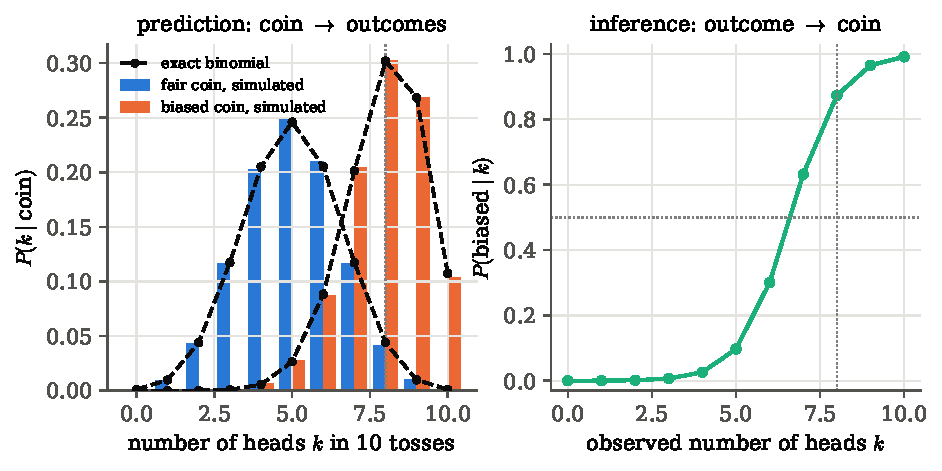
\includegraphics[width=\linewidth]{figures/ch00/coin_two_directions.pdf}
\caption{Left, prediction: each coin, tossed ten times over and over, spreads
its outcomes over $k=0,\dots,10$. Bars are simulated frequencies, dashed
curves the exact binomial probabilities; the dotted line marks the observed
$k=8$. Right, inference: for each possible observation $k$, the probability
that the coin was the biased one. The curve crosses the prior value $\frac12$
between $k=6$ and $k=7$, where the two coins explain the data about equally
well.}
\label{0a:fig:coin-two-directions}
\end{figure}

The forward number $\Prob(E\given H)$ and the backward number
$\Prob(H\given E)$ can be far apart. The classic case is a medical test, and
it goes through the same four steps. A disease affects $1\%$ of people. A test
detects it with probability $0.95$ and gives a false positive with probability
$0.10$.

\emph{The event.} A patient tests positive, written $+$.

\emph{What could have produced it?} The one thing we do not know is whether
the patient is ill. So there are two candidates: the patient has the disease
($D$), or does not ($D^c$).

\emph{How probable was the event under each?} If the patient is ill, the test
catches it $95\%$ of the time: $\Prob(+\given D)=0.95$. If the patient is
healthy, a positive result is a false alarm, which happens $10\%$ of the time:
$\Prob(+\given D^c)=0.10$.

\emph{Only then the priors, and the normalisation.} Before the test, the
patient was ill with probability $0.01$ and healthy with probability $0.99$.
Bayes' theorem \eqref{0a:eq:bayes} gives
\[
  \Prob(D\given +)=\frac{0.95\times0.01}{0.95\times0.01+0.10\times0.99}
  =\frac{0.0095}{0.1085}=0.0876 .
\]

\begin{pitfall}[$\Prob(E\given H)$ is not $\Prob(H\given E)$]
The two numbers answer different questions and can be wildly different. For
the positive test, the forward number $\Prob(+\given D)=0.95$ is not the
answer to ``is the patient ill?''; the answer is $\Prob(D\given +)=0.0876$.
Swapping the two conditionals is the ``prosecutor's fallacy''. Its statistical
twin appears in \cref{ch:04}: a $p$-value is \emph{not} the probability that
the null hypothesis is true.
\end{pitfall}

The lesson is not in the arithmetic. A positive result can come by two paths:
through the disease, or through a false alarm on a healthy person. Each
healthy person is unlikely to take the false-alarm path, but there are 99
healthy people for every ill one. The positive result favours the disease only
by the factor $\Prob(+\given D)/\Prob(+\given D^c)=0.95/0.10=9.5$. A factor of
$9.5$ acting on a prior of $1\%$ leaves the posterior below $10\%$, far from
the $95\%$ that the test's sensitivity suggests (\cref{5a:sec:shrink} draws it
to scale).

\paragraph{Two meanings of ``prediction''.}
In this chapter ``prediction'' means the forward direction, $H\to E$.
Statistics and machine-learning books also use the word for guessing a
\emph{new} data point (a regression output, a class label) after learning from
old data. That second kind of prediction is part of inference, because it
starts from data. When Wasserman lists ``prediction, classification,
clustering, and estimation'' as special cases of inference, he means the
second sense.

\providecommand{\zeroaIconLSS}{\tikz[baseline=0.1cm,x=1cm,y=1cm]{%
  \foreach \x/\y in {0.1/0.1,0.25/0.5,0.4/0.2,0.55/0.6,0.7/0.15,0.85/0.45,0.3/0.3,0.65/0.35,0.9/0.1,0.15/0.62}
    {\fill[formblue!80] (\x,\y) circle (0.9pt);}
  \draw[bdryred,thick] (0.5,0.35) circle (0.27);}}
\providecommand{\zeroaIconReal}{\tikz[baseline=0.1cm,x=1cm,y=1cm]{%
  \draw[formblue,thick] plot[domain=0.0:1.0,samples=30,smooth] (\x,{0.55*exp(-2.2*\x)+0.08});
  \foreach \x/\y in {0.1/0.47,0.3/0.39,0.5/0.26,0.7/0.21,0.9/0.17}
    {\draw[black] (\x,\y-0.06)--(\x,\y+0.06); \fill (\x,\y) circle (1pt);}
  \draw[softgray] (0,0)--(1.0,0);}}
\providecommand{\zeroaIconTree}{\tikz[baseline=0.2cm,x=1cm,y=1cm]{%
  \draw[softgray,thin] (0,0.3)--(0.45,0.55) (0,0.3)--(0.45,0.05)
    (0.45,0.55)--(0.95,0.68) (0.45,0.05)--(0.95,-0.08);
  \draw[bdryred,thick] (0.45,0.55)--(0.95,0.42) (0.45,0.05)--(0.95,0.18);
  \fill (0,0.3) circle (1pt);}}
\providecommand{\zeroaIconHist}{\tikz[baseline=0.1cm,x=1cm,y=1cm]{%
  \foreach \i/\h in {0/0.03,1/0.18,2/0.45,3/0.6,4/0.45,5/0.18,6/0.03}
    {\fill[formblue!70] (0.14*\i,0) rectangle ({0.14*\i+0.11},\h);}
  \draw[softgray] (-0.03,0)--(1.0,0);}}
\providecommand{\zeroaIconEst}{\tikz[baseline=0.1cm,x=1cm,y=1cm]{%
  \draw[formblue,thick] plot[domain=0.05:1.0,samples=40,smooth]
    (\x,{0.6*exp(-((\x-0.58)^2)/(2*0.11^2))});
  \draw[black,dashed] (0.5,0)--(0.5,0.68);
  \draw[softgray] (0,0)--(1.0,0);}}
\providecommand{\zeroaIconTest}{\tikz[baseline=0.1cm,x=1cm,y=1cm]{%
  \fill[bdryred!70] plot[domain=0.75:1.0,samples=15,smooth]
    (\x,{0.6*exp(-((\x-0.4)^2)/(2*0.16^2))}) -- (1.0,0) -- (0.75,0) -- cycle;
  \draw[formblue,thick] plot[domain=0.0:1.0,samples=40,smooth]
    (\x,{0.6*exp(-((\x-0.4)^2)/(2*0.16^2))});
  \draw[bdryred,thick] (0.75,0)--(0.75,0.35);
  \draw[softgray] (0,0)--(1.0,0);}}
\providecommand{\zeroaIconBayes}{\tikz[baseline=0.1cm,x=1cm,y=1cm]{%
  \draw[softgray,dashed] plot[domain=0.0:1.0,samples=30,smooth]
    (\x,{0.25*exp(-((\x-0.45)^2)/(2*0.3^2))});
  \draw[formblue,thick] plot[domain=0.3:1.0,samples=40,smooth]
    (\x,{0.65*exp(-((\x-0.65)^2)/(2*0.08^2))});
  \draw[softgray] (0,0)--(1.0,0);}}
\providecommand{\zeroaIconMC}{\tikz[baseline=0.05cm,x=1cm,y=1cm]{%
  \draw[softgray] (0,0) rectangle (0.7,0.7);
  \draw[formblue] (0.7,0) arc (0:90:0.7);
  \foreach \x/\y in {0.1/0.2,0.3/0.5,0.55/0.15,0.62/0.6,0.2/0.62,0.45/0.35,
                     0.66/0.4,0.15/0.4,0.35/0.1,0.5/0.55,0.27/0.3,0.6/0.27}
    {\fill[fibreorange] (\x,\y) circle (0.7pt);}}}
\providecommand{\zeroaIconMCMC}{\tikz[baseline=0.05cm,x=1cm,y=1cm]{%
  \draw[softgray,rotate around={30:(0.5,0.35)}] (0.5,0.35) ellipse (0.45 and 0.2);
  \draw[tangentgreen,thin] (0.05,0.02)--(0.2,0.12)--(0.28,0.3)--(0.42,0.26)
    --(0.5,0.4)--(0.62,0.44)--(0.55,0.33)--(0.7,0.5)--(0.78,0.46)--(0.66,0.38)
    --(0.8,0.6);
  \fill[tangentgreen] (0.05,0.02) circle (0.8pt);}}
\providecommand{\zeroaIconFisher}{\tikz[baseline=0.05cm,x=1cm,y=1cm]{%
  \draw[softgray,->] (0,0)--(1.0,0); \draw[softgray,->] (0,0)--(0,0.7);
  \draw[formblue,thick,rotate around={-35:(0.5,0.35)}] (0.5,0.35) ellipse (0.36 and 0.12);
  \fill[formblue] (0.5,0.35) circle (0.8pt);}}
\providecommand{\zeroaIconField}{\tikz[baseline=0.05cm,x=1cm,y=1cm]{%
  \draw[softgray,->] (0,0)--(1.0,0); \draw[softgray,->] (0,0)--(0,0.7);
  \draw[formblue,thick] plot[domain=0.05:0.95,samples=40,smooth]
    (\x,{0.12+0.45*exp(-((\x-0.3)^2)/(2*0.08^2))+0.2*exp(-((\x-0.62)^2)/(2*0.06^2))});}}
\providecommand{\zeroaIconTopo}{\tikz[baseline=0.05cm,x=1cm,y=1cm]{%
  \fill[bdryred!60] (0.15,0.45) circle (0.12);
  \fill[bdryred!60] (0.32,0.15) circle (0.1);
  \fill[bdryred!60,even odd rule] (0.72,0.35) circle (0.26) (0.72,0.35) circle (0.12);}}

\section{The questions the book answers}\label{0a:sec:questions}

One coin already raises many different questions, and each needs its own
tool. Keep the coin from the magic shop of \cref{0a:sec:two-directions}, but
forget the drawer. Now there is a single coin whose heads probability $p$ is
unknown, and we may toss it as often as we like.
\emph{How likely is 8 heads if $p=\frac12$?} is a forward calculation.
\emph{What is our best guess for $p$, and how wrong might it be?} is
estimation. \emph{Is 8 heads in 10 surprising for a fair coin?} is a test.
\emph{Which values of $p$ are plausible now?} is Bayesian inference.
\emph{Could we get any of these numbers by simulation instead of algebra?} is
Monte Carlo. \emph{How many tosses would we need to pin $p$ down to $\pm 0.01$?}
is a Fisher forecast. Each question has its own object that answers it, and
each has its own chapter. If we keep the questions apart, then for any tool we
can say which question it answers.

\paragraph{Same system, different measurements.}
A physicist knows this from the lab. One pendulum supports many experiments.
We can measure its period, estimate $g$ from the period, test whether the
period depends on the amplitude, or forecast how precisely a longer run would
pin down $g$. The pendulum stays the same. What changes is the question, and
with it the quantity we must compute. Probability tools work the same way: the
model stays fixed, and each tool computes the quantity that answers one
question about it.

\paragraph{The questions in words.}
Before any formula, each kind of question can be said in one sentence.
\begin{enumerate}[leftmargin=2em]
  \item \emph{Forward:} if the hypothesis is true, how often does this outcome occur?
  \item \emph{Spread:} what values can a random quantity take, and how are they distributed?
  \item \emph{Estimation:} what value of the parameter do the data point to, and how far off is that guess likely to be?
  \item \emph{Testing:} if only chance were at work, would a result like this, or one even more extreme in the same direction, be something we would reasonably expect?
  \item \emph{Bayesian inference:} which parameter values could have produced the data, and how probable is each one?
  \item \emph{Simulation:} can we get the answer to any of these by drawing random numbers, when the algebra is too hard?
  \item \emph{Forecasting:} before the experiment is run, how well could it measure the parameter?
  \item \emph{Choosing the summary:} which property of a field (a map, a density) carries the physics, and does it survive the nuisance effects of observation?
\end{enumerate}

The table below is the map of the book. Each row gives one question, the
object that answers it, and the chapter where that object is built. The
pictogram on the left of each row is a miniature of the central figure of that
chapter, the picture to remember for the row.

\begin{taxonomy}[which object answers which question]
\footnotesize
\renewcommand{\arraystretch}{1.35}
\begin{tabularx}{\linewidth}{@{}>{\centering\arraybackslash}m{1.15cm}
  >{\raggedright\arraybackslash}X >{\raggedright\arraybackslash}p{4.3cm}
  >{\centering\arraybackslash}m{1.0cm}@{}}
\toprule
& \textbf{The question, in words} & \textbf{The object that answers it} & \textbf{Ch.}\\
\midrule
\zeroaIconTree & How likely is this event, if the situation is as assumed? Which paths lead to it? &
  $\Prob(E\given H)$, summed over the paths of a probability tree & \ref{ch:01}\\
\zeroaIconHist & What values can a random quantity take, and how are they spread? &
  a distribution: pmf or pdf, CDF, mean and variance (binomial, Poisson, Gaussian, \dots) & \ref{ch:02}\\
\zeroaIconEst & What value of the parameter do the data point to, and how far off is that guess? &
  an estimator $\hat\theta$, its bias and variance, i.e.\ its sampling distribution; the likelihood $\Like(\theta)$ & \ref{ch:03}\\
\zeroaIconTest & If $\Hnull$ (the case whose distribution we know: ``it happened by chance'') were true, would a result like this, or more extreme in this direction, be expected? &
  a test statistic and its $p$-value, the tail probability under $\Hnull$ & \ref{ch:04}\\
\zeroaIconBayes & Which parameter values (or models) could have produced the data, and how probable is each? &
  the posterior $p(\params\given\data)\propto\Like(\params)\,p(\params)$; the evidence $Z$ for comparing models & \ref{ch:05}\\
\zeroaIconMC & What is the distribution of a quantity too complicated to compute by hand? &
  many simulated realisations; histograms and averages, with error $\propto 1/\sqrt N$ & \ref{ch:06}\\
\zeroaIconField & How do we summarise a random field (a sky map), and how does the summary fluctuate? &
  correlation function $\xi(r)$, power spectrum $P(k)$, $\Cell$ and its estimator $\Chat$ & \ref{ch:07}\\
\zeroaIconMC & How do a mask, noise and a beam change the sampling distribution of the summary? &
  Monte Carlo as the research instrument: simulated skies through the observation pipeline & \ref{ch:08}\\
\zeroaIconMCMC & How do we draw samples from a posterior in many dimensions without ever normalising it? &
  a Markov chain: a \emph{biased} random walker that lingers where the posterior is high & \ref{ch:09}\\
\zeroaIconFisher & Before the experiment, how well could it measure $\params$? &
  the Fisher matrix $\Fish$; forecast errors $\sigma_i\ge\sqrt{(\Fish^{-1})_{ii}}$ & \ref{ch:10}\\
\zeroaIconLSS & What do the positions and motions of galaxies say about how the Universe expands and how structure grows? &
  galaxy catalogues: $\xi(s)$ and $P(k)$ with weights and windows, the BAO ruler, peculiar velocities & \ref{ch:11}\\
\zeroaIconTopo & Is there information in how the structures of a field are connected, robust to nuisance effects? &
  excursion sets, Betti numbers, Euler characteristic, persistence: new random observables $S$ with a $P(S\given\theta)$ & \ref{ch:12}\\
\zeroaIconReal & Does the whole chain survive contact with real data? &
  complete analyses of Planck, SDSS and collider data, each reproducing a published result & \ref{ch:13}\\
\bottomrule
\end{tabularx}
\par\medskip\noindent
\Cref{ch:14} puts the rows back together: given a new problem, which row does
it belong to?
\end{taxonomy}

Most of the rows can be tried on the coin in a few lines. Four of them need a
new idea: estimation, testing, Monte Carlo and forecasting. Two definitions
carry all four.

\begin{workdef}[estimator, sampling distribution, $p$-value]
An \newterm{estimator} is a recipe that turns data into a guess for a
parameter, $\hat\theta=\hat\theta(\data)$ \unpack{a function of the data only,
e.g.\ $\hat p=k/n$, the fraction of heads}. Because the data are random, so is
$\hat\theta$. Its distribution over imagined repetitions of the whole
experiment is its \newterm{sampling distribution} \unpack{the histogram of
$\hat\theta$ if the experiment were rerun many times with the same true
$\theta$}. Its \newterm{bias} is $\E[\hat\theta]-\theta$ and its spread is
$\Var(\hat\theta)$.

A \newterm{null hypothesis} $\Hnull$ is a hypothesis whose sampling distribution
we know \unpack{``nothing but chance'', e.g.\ a fair coin}. Given an observed
value $t_{\rm obs}$ of a statistic $T$, the \newterm{$p$-value} is
\begin{equation}
  \pval=\Prob\big(T\ge t_{\rm obs}\given \Hnull\big),
  \label{0a:eq:pvalue}
\end{equation}
the probability, computed under $\Hnull$, of a result like the observed one
\emph{or even more in this direction} \unpack{here, larger values of $T$
count as further out}. We can compute it only because ``pure chance'' is the
one case whose distribution we have in hand. For a fair coin we know exactly
how often each head count turns up. A small $\pval$ says that, if the coin
really were fair, a result this far out would be a surprise (\cref{ch:04}).
\end{workdef}

\zeroaEx{the scatter of a fraction}
\label{0a:ex:mc-error}
The natural guess for $p$ is the fraction of heads. The question is whether
this guess is right on average, and how far it typically misses. Toss the coin
$n$ times and let $x_i=1$ if toss $i$ is heads and $x_i=0$ if it is tails. The
number of heads is $k=\sum_i x_i$, so the estimator is
$\hat p=k/n=\frac1n\sum_i x_i$. Its mean and variance are
\begin{align*}
  \E[\hat p] &\eqby{1} \frac1n\sum_{i=1}^n\E[x_i] \eqby{2} \frac1n\,n\,p = p,\\
  \Var(\hat p) &\eqby{3} \frac1{n^2}\sum_{i=1}^n\Var(x_i)
   \eqby{4} \frac1{n^2}\,n\,\big(\E[x_i^2]-\E[x_i]^2\big)
   \eqby{5} \frac{p-p^2}{n}=\frac{p(1-p)}{n} .
\end{align*}
\begin{explain}
  \item The expectation of a sum is the sum of expectations, and constants come out.
  \item $\E[x_i]=1\cdot p+0\cdot(1-p)=p$.
  \item For \emph{independent} tosses the variance of a sum is the sum of variances; a constant $c$ comes out as $c^2$.
  \item Definition of the variance, $\Var(x)=\E[x^2]-\E[x]^2$.
  \item $x_i^2=x_i$ because $x_i$ is $0$ or $1$, so $\E[x_i^2]=p$.
\end{explain}
So $\hat p$ is \newterm{unbiased}: on average it gives the true $p$. Its
standard deviation, the typical miss, is $\sqrt{p(1-p)/n}$. For $p=0.8$ this
is $0.126$ at $n=10$ and $0.040$ at $n=100$. The same algebra applies to
\emph{any} fraction of $N$ independent trials that each succeed with
probability $q$. That is why a Monte Carlo estimate of a probability $q$ from
$N$ simulated trials has error $\sqrt{q(1-q)/N}$.

\zeroaEx{the $p$-value of 8 heads}
\label{0a:ex:pvalue}
\emph{The observation.} Ten tosses gave 8 heads.
\emph{The question.} If the coin were fair, would 8 heads, or more than 8 heads, be something we would reasonably expect?
\emph{The pieces.} The null hypothesis is $\Hnull$: $p=\frac12$. The statistic
is the number of heads, $T=k$, and ``more extreme'' means more heads. Then
\begin{align*}
  \Prob(K\ge 8\given\Hnull)
  &\eqby{1} \Prob(8)+\Prob(9)+\Prob(10)
   \eqby{2} \frac{\binom{10}{8}+\binom{10}{9}+\binom{10}{10}}{2^{10}}
   = \frac{45+10+1}{1024}=\frac{56}{1024}=0.0547 .
\end{align*}
\begin{explain}
  \item ``This or more extreme in this direction'': the outcomes $8,9,10$ are exclusive, so their probabilities add.
  \item Binomial probabilities with $p=\frac12$ (\cref{0a:ex:forward}): every sequence has probability $2^{-10}$.
\end{explain}
About $5\%$ of fair ten-toss runs give 8 heads or more
(\cref{0a:fig:pvalue}). That is mildly surprising, not damning. The $p$-value
used only the distribution under $\Hnull$; it never mentioned the biased coin.
It is \emph{not} $\Prob(\Hnull\given\text{data})$, the probability that the
coin is fair. In the drawer story of \cref{0a:sec:two-directions} (equal
numbers of fair and biased coins) that number was $\Prob(F\given 8)=0.127$, the
answer to a different question.

\begin{figure}[htbp]
\centering
\begin{tikzpicture}
\begin{axis}[width=10cm,height=4.6cm,ybar,bar width=0.55cm,ymin=0,ymax=0.27,
  xtick={0,...,10},xlabel={number of heads $k$ in 10 tosses of a fair coin},
  ylabel={$\Prob(k\given\Hnull)$},axis x line*=bottom,axis y line*=left,
  enlarge x limits=0.06,tick label style={font=\footnotesize},
  label style={font=\small}]
\addplot[bar shift=0pt,fill=formblue!45,draw=formblue] coordinates
  {(0,0.000977) (1,0.009766) (2,0.043945) (3,0.117188) (4,0.205078) (5,0.246094)
   (6,0.205078) (7,0.117188)};
\addplot[bar shift=0pt,fill=bdryred!70,draw=bdryred] coordinates
  {(8,0.043945) (9,0.009766) (10,0.000977)};
\end{axis}
\node[font=\small,bdryred,anchor=west] at (6.9,2.2) {$56/1024=0.055$};
\end{tikzpicture}
\caption{The null distribution for ten tosses of a fair coin. The red bars are
the observed $k=8$ and the outcomes more extreme in the same direction; their
total height is the $p$-value. The blue bars never enter.}
\label{0a:fig:pvalue}
\end{figure}

\zeroaEx{a forecast before any toss: the Fisher information}
\label{0a:ex:fisher}
The question is asked before any toss: how precisely \emph{could} $n$ tosses
measure $p$? The answer depends on how sharply the data single out one value
of $p$. The likelihood of one particular sequence with $k$ heads is
$\Like(p)=p^k(1-p)^{n-k}$, so its logarithm is
$\ln\Like(p)=k\ln p+(n-k)\ln(1-p)$. A log-likelihood with a sharp peak pins
$p$ down; a flat one does not. The \newterm{Fisher information} measures the
sharpness. It is minus the expected curvature of $\ln\Like$ at the true $p$:
\begin{align*}
  I(p) &\eqby{1} -\E\!\left[\frac{\dd^2\ln\Like}{\dd p^2}\right]
   \eqby{2} \E\!\left[\frac{k}{p^2}+\frac{n-k}{(1-p)^2}\right]
   \eqby{3} \frac{np}{p^2}+\frac{n(1-p)}{(1-p)^2}
   = \frac np+\frac n{1-p}
   = \frac{n}{p(1-p)} .
\end{align*}
\begin{explain}
  \item Definition (\cref{ch:10}): a sharply curved log-likelihood pins the parameter down.
  \item $\frac{\dd}{\dd p}\ln\Like=\frac kp-\frac{n-k}{1-p}$; differentiate again and change sign.
  \item $\E[k]=np$ and $\E[n-k]=n(1-p)$.
\end{explain}
The Cram\'er--Rao bound (\cref{ch:03,ch:10}) says that no unbiased estimator
can beat $\Var(\hat\theta)\ge 1/I$. Here $1/I=p(1-p)/n$, exactly the variance of
$\hat p$ found in \cref{0a:ex:mc-error}. So the fraction of heads is as good
as any unbiased guess can be. The forecast needs no data, only an assumed
$p$. To reach a standard deviation $\sigma_p=0.01$ at $p\approx0.8$ we need
$n=p(1-p)/\sigma_p^2=0.16/10^{-4}=1600$ tosses.

\paragraph{What this bought us.}
The same coin gave three different numbers: a spread $\sqrt{p(1-p)/n}$
(estimation), a tail probability $0.055$ (testing) and a required number of
tosses, $1600$ (forecasting). None of them is a posterior. Each answers its
own row of the table. Confusing the rows is the most common error in applied
statistics.

\begin{pitfall}[what a $p$-value and a confidence interval do \emph{not} say]
A $p$-value of $0.055$ does not mean ``the coin is fair with probability
$0.055$''. It is $\Prob(\text{data this extreme}\given\Hnull)$, a forward
number. Likewise, a $95\%$ confidence interval is a recipe that covers the
true value in $95\%$ of repetitions of the experiment; it is not an interval
that contains the parameter with probability $95\%$. Only the posterior of
\cref{ch:05} makes probability statements about parameters.
\end{pitfall}

\subsection*{The questions in code}

The script \pyname{02_coin_questions.py} checks two of these answers by brute
force. The key lines are:

\pyfile[firstline=23,lastline=37]{code/ch00/02_coin_questions.py}{Estimation and a $p$-value by simulation}

The first block reruns the whole ten-toss experiment, and the hundred-toss
one, $50\,000$ times with the true $p=0.8$, and keeps each $\hat p$. That list
is a sample from the sampling distribution of $\hat p$. The second block is
\cref{0a:ex:pvalue} in one line. The third block simulates fair experiments.
In it, \pyname{np.cumsum(fair >= K_OBS)} counts, for every $N$ at once, how
many of the first $N$ experiments were as extreme as the observed 8 heads.
The last line is the error bar $\sqrt{q(1-q)/N}$ of \cref{0a:ex:mc-error}.

The run confirms both calculations. The standard deviation of $\hat p$ is
$\QSdTen$ at $n=10$ (theory $\QSdTenTh$) and $\QSdHundred$ at $n=100$ (theory
$\QSdHundredTh$). The mean at $n=10$ is $\QMeanTen$, so the estimator is
unbiased, as derived. The Monte Carlo $p$-value is $\QPmcHundred$ after
$N=\QNhundred$ experiments and $\QPmcMillion\pm\QSigmaMillion$ after $10^6$,
against the exact $\QPexact$.

\begin{figure}[htbp]
\centering
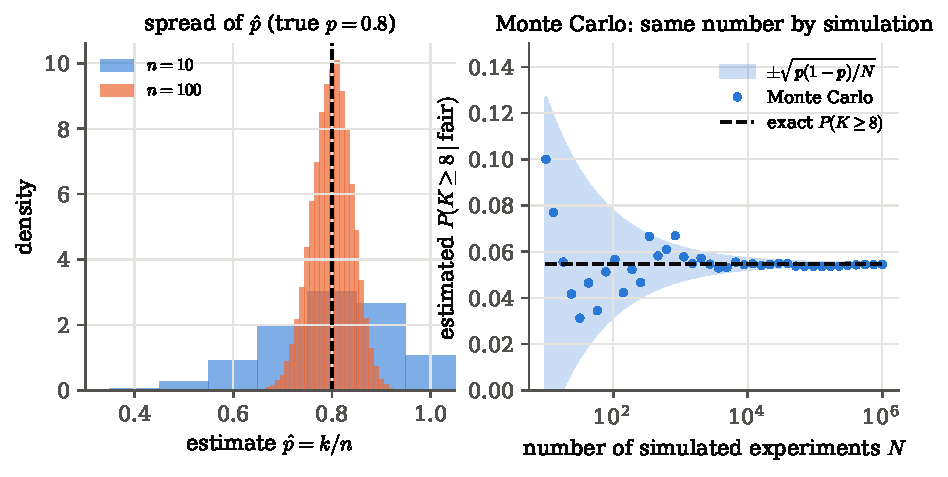
\includegraphics[width=\linewidth]{figures/ch00/coin_questions.pdf}
\caption{Left: the sampling distribution of $\hat p=k/n$ for a coin with
$p=0.8$. With 10 tosses the guesses spread over most of the interval; with 100
they crowd around the true value, ten times more tightly in variance. Right:
the Monte Carlo estimate of $\Prob(K\ge8\given$fair$)$ as the number of
simulated experiments grows. The points wander inside the shaded
$\pm\sqrt{p(1-p)/N}$ band, which narrows onto the exact value.}
\label{0a:fig:coin-questions}
\end{figure}

\begin{inpractice}[verification versus research]
Monte Carlo has two uses. Here it only \emph{verifies} a number we could
compute exactly, $56/1024$; the first use is to check theory and code against
each other. The second use is as the \emph{research instrument}, where no
exact answer exists. Suppose the ``coin'' were a CMB sky seen through a
galactic mask, with noise and a beam. Nobody can write down the distribution
of the measured power spectrum. Instead one simulates thousands of skies and
makes a histogram. The code is the same: draw, compute the statistic, count.
\Cref{ch:06} builds the first use, \cref{ch:08} the second.
\end{inpractice}

\paragraph{The same idea under different names.}
The vocabulary changes between communities, but the ideas do not. What
statisticians call \emph{estimation}, the machine-learning literature calls
\emph{learning}. The observed values $(X_i,Y_i)$ are there the \emph{training
sample}. The inputs $X_i$ are \emph{covariates} in one language and
\emph{features} in the other. A few more terms recur. A \emph{hypothesis} is a
subset of the parameter space. A \emph{confidence interval} is a recipe that
covers the unknown value with a stated frequency. \emph{Bayesian inference}
means using data to update beliefs, whereas \emph{frequentist inference}
collects the methods whose long-run frequency behaviour is guaranteed
\mainref{p.~xi}. Prediction in the second sense of
\cref{0a:sec:two-directions}, together with classification, clustering and
estimation, counts as a special case of inference \mainref{p.~ix}. Only the
Bayesian rows of the table above (\cref{ch:05,ch:09}) share out credibility
among parameter values \srcref{Kruschke}{p.~15}. The estimation and testing
rows instead describe how a \emph{procedure} behaves over repeated
experiments. The null hypothesis is the case whose distribution we know,
because we assume the result happened by chance \mainref{p.~149}.

\section{The pipeline: from a physical model to a statement about physics}\label{0a:sec:pipeline}

Real data are never fed into Bayes' theorem whole; they are compressed first.
A Planck temperature map at the resolution used for cosmology has about
$5\times10^{7}$ pixels. The model we want to test, $\Lambda$CDM, has six
parameters. Nobody writes Bayes' theorem directly for fifty million correlated
pixels. Instead the map is compressed into its angular power spectrum $\Chat$,
about $2500$ numbers, and those are compared with the theory. Each step of
this is a choice. First we decide that the power spectrum is the information
that matters. Then we work out how $\Chat$ fluctuates from one sky to another.
Only then do we infer the six parameters. Written out as one pipeline, this
chain of choices has an arrow for every tool in the book. Knowing which arrow
we are on is the fastest way to know what a tool is for.

\paragraph{Microstates and macrostates.}
Statistical mechanics works the same way. A gas has $10^{23}$ momenta, but we
never infer anything from the full microstate. We compress it into a few
macroscopic summaries (pressure, energy, magnetisation). Fluctuation theory
then tells us how much those summaries scatter; for example, the energy of a
system at temperature $T$ with heat capacity $C_V$ fluctuates by
$\langle\Delta E^2\rangle=k_BT^2C_V$. A summary is chosen for two reasons: it
carries the physics we care about, and its fluctuations can be calculated.
Data analysis makes the same two demands of every summary statistic.

\paragraph{Six stages, six questions.}
The whole book runs along one chain, drawn in \cref{0a:fig:pipeline}:
\begin{equation}
\boxed{\begin{array}{l}
\text{a theory with parameters }\params\;\rightarrow\;\text{the map or data set it produces}\\[2pt]
\qquad\rightarrow\;\text{decide which features of the data carry the physics}\\[2pt]
\qquad\rightarrow\;\text{compress the data into a statistic }S
\;\rightarrow\;\text{work out how }S\text{ scatters, }P(S\given\params)\\[2pt]
\qquad\rightarrow\;\text{say what the observed }S\text{ tells us about }\params
\end{array}}
\label{0a:eq:workflow}
\end{equation}
In symbols, the last two stages are $P(S\given\theta)$ and
$P(\theta\given S)\propto P(S\given\theta)P(\theta)$, where $\theta$ stands for
the parameters $\params$. The stages answer different kinds of question. The
choice of summary decides what should be measured. The last two stages decide
how the uncertainty in that measurement carries over to the parameters. The
same chain applies whether the data vector holds pixelised CMB temperatures or
measured bandpowers $C_\ell$, and whatever the number $M$ of model parameters.
Each stage is a question.
\begin{enumerate}[leftmargin=2em]
  \item \emph{Physical model:} what theory, with which parameters $\params$, could have produced the data?
  \item \emph{Field or dataset:} what exactly did the instrument record, and how does it depend on $\params$ and on noise?
  \item \emph{What information matters:} which property of the data is sensitive to $\params$, and which is only nuisance?
  \item \emph{Summary:} which function $S[\data]$ of the data keeps that property and discards the rest?
  \item \emph{Sampling distribution:} if the experiment were repeated with the same $\params$, how would $S$ scatter? That is $P(S\given\params)$.
  \item \emph{Infer physics:} given the one $S$ we observed, which $\params$ are plausible? That is $P(\params\given S)\propto P(S\given\params)P(\params)$.
\end{enumerate}
Stages 1 to 5 are the forward direction of \cref{0a:sec:two-directions}.
Stage 6 is the backward direction.

\begin{figure}[htbp]
\centering
\begin{tikzpicture}[
  stage/.style={draw=accent,thick,rounded corners=2pt,fill=ideabg,align=center,
                font=\small,text width=5.4cm,minimum height=0.95cm},
  flow/.style={->,thick,accent},
  chap/.style={font=\footnotesize,align=left,anchor=west,text width=5.3cm}]
  \node[stage] (m) at (0,0)     {physical model, parameters $\params$\\[-1pt]\footnotesize $\Lambda$CDM, a signal strength $\mu$, a coin's $p$};
  \node[stage] (d) at (0,-1.7)  {field or dataset $\data$\\[-1pt]\footnotesize a sky map, event counts, a strain record};
  \node[stage] (c) at (0,-3.4)  {decide which features\\ carry the physics};
  \node[stage] (s) at (0,-5.1)  {compress into a statistic $S[\data]$\\[-1pt]\footnotesize $k$, $\Chat$, $\xi(r)$, $\beta_0(\nu)$, \dots};
  \node[stage] (p) at (0,-6.8)  {work out how $S$ scatters: $P(S\given\params)$};
  \node[stage,fill=takebg,draw=tangentgreen] (i) at (0,-8.5) {what $S$ says about $\params$: $P(\params\given S)\propto P(S\given\params)\,P(\params)$};
  \draw[flow] (m) -- (d); \draw[flow] (d) -- (c); \draw[flow] (c) -- (s);
  \draw[flow] (s) -- (p); \draw[flow] (p) -- (i);
  \node[chap] at (3.2,-0.85) {\textbf{simulate the forward model:}\\ probability and distributions (Ch.~\ref{ch:01}, \ref{ch:02}), random fields (Ch.~\ref{ch:07}), Monte Carlo (Ch.~\ref{ch:06})};
  \node[chap] at (3.2,-2.55) {\textbf{which information?} phases and morphology that $\Cell$ discards (Ch.~\ref{ch:07}, \ref{ch:12})};
  \node[chap] at (3.2,-4.25) {\textbf{build the summary:} estimators (Ch.~\ref{ch:03}), $\Chat$ (Ch.~\ref{ch:07}), Betti numbers, $\chi$ (Ch.~\ref{ch:12})};
  \node[chap] at (3.2,-5.95) {\textbf{how does $S$ scatter?} error propagation (Ch.~\ref{ch:03}), null distributions (Ch.~\ref{ch:04}), Monte Carlo through mask, noise, beam (Ch.~\ref{ch:06}, \ref{ch:08})};
  \node[chap] at (3.2,-7.65) {\textbf{turn scatter into constraints:} tests (Ch.~\ref{ch:04}), Bayes (Ch.~\ref{ch:05}), MCMC (Ch.~\ref{ch:09}), Fisher (Ch.~\ref{ch:10})};
  \draw[->,thick,softgray,dashed] (i.west) -- ++(-0.6,0) |- (m.west);
  \node[font=\footnotesize,softgray,align=right,anchor=east] at (-3.6,-4.25) {check the\\ model, then\\ design the\\ next\\ experiment};
\end{tikzpicture}
\caption{The pipeline of the whole book. Boxes are the stages; the notes on
the right say which chapters serve the step from one box to the next. The
top four boxes are forward modelling and a choice, the fifth is probability
theory applied to that choice, and only the last box is inference. The dashed
loop is the step statisticians call a posterior predictive check: simulate
data from the inferred model and ask whether they look like the real data.}
\label{0a:fig:pipeline}
\end{figure}

One step of the pipeline is not mathematics: choosing what information
matters. It is a physics decision, and \cref{0a:sec:summaries} takes it up.
The next step, building the summary, does have a precise test: it tells us
when compressing the data loses nothing.

\begin{workdef}[summary statistic, sampling distribution, sufficiency]
A \newterm{summary statistic} is any function $S=S[\data]$ of the data
\unpack{a number or a short vector computed from the data alone, e.g.\ the
number of heads $k$}. Its \newterm{sampling distribution} $P(S\given\params)$
is the distribution of $S$ over repetitions of the experiment with the
parameters held fixed \unpack{the histogram of $S$ over many simulated
universes that share the same $\params$}. The summary is \newterm{sufficient}
for $\params$ if the likelihood depends on the data only through $S$:
\begin{equation}
  P(\data\given\params)=g\big(S[\data],\params\big)\,h(\data)
  \label{0a:eq:factorisation}
\end{equation}
\unpack{$h$ may depend on the data but not on $\params$, so it cancels from
every posterior and every likelihood ratio}. Then $P(\params\given\data)
=P(\params\given S)$: nothing about $\params$ was thrown away.
\end{workdef}

The coin shows how the test works. The data are the whole sequence
$x_1,\dots,x_n$ of zeros and ones ($x_i=1$ for heads, as in
\cref{0a:ex:mc-error}). Is the number of heads enough, or does the order of
the tosses also tell us something about $p$? Write down the probability of the
sequence:
\begin{align}
  P(x_1,\dots,x_n\given p)
  &\eqby{1} \prod_{i=1}^{n} p^{x_i}(1-p)^{1-x_i} \nonumber\\
  &\eqby{2} p^{\sum_i x_i}\,(1-p)^{\,n-\sum_i x_i}
   \eqby{3} p^{k}(1-p)^{n-k} .
  \label{0a:eq:coin-suff}
\end{align}
\begin{explain}
  \item The tosses are independent; one toss gives $p$ if $x_i=1$ and $1-p$ if $x_i=0$, which is what $p^{x_i}(1-p)^{1-x_i}$ says.
  \item Products of powers of the same base add their exponents.
  \item $k=\sum_i x_i$ is the number of heads.
\end{explain}
The sequence enters only through $k$. So \eqref{0a:eq:coin-suff} has the form
\eqref{0a:eq:factorisation} with $S=k$, $g=p^k(1-p)^{n-k}$ and $h=1$, and the
order of the tosses carries no information about $p$. The sampling
distribution of the summary $k$ is the binomial of \cref{0a:ex:forward}. The
last stage puts it into Bayes' theorem.

\zeroaEx{the coin through the whole pipeline}
\label{0a:ex:coin-pipeline}
The last stage asks: after $k$ heads in $n$ tosses, which values of the heads
probability $p$ are plausible, and how plausible is each? Now $p$ can be any
number in $[0,1]$, not one of two coins. Take a flat prior, $p(p)=1$ on
$[0,1]$, which treats every value as equally plausible beforehand. The
posterior for $p$ is then
\begin{align*}
  p(p\given k)
  &\eqby{1} \frac{P(k\given p)\cdot 1}{\int_0^1 P(k\given p')\,\dd p'}
   \eqby{2} \frac{p^{k}(1-p)^{n-k}}{\int_0^1 p'^{k}(1-p')^{n-k}\,\dd p'}
   \eqby{3} \frac{(n+1)!}{k!\,(n-k)!}\,p^{k}(1-p)^{n-k} .
\end{align*}
\begin{explain}
  \item Bayes' theorem for a continuous parameter: the sum over hypotheses in \eqref{0a:eq:bayes} becomes an integral.
  \item The factor $\binom nk$ does not depend on $p$ and cancels between numerator and denominator.
  \item The Beta integral $\int_0^1 p^a(1-p)^b\,\dd p=\frac{a!\,b!}{(a+b+1)!}$ for non-negative integers $a,b$ (proved by $b$ integrations by parts, each moving one power from $(1-p)$ to $p$).
\end{explain}
Where is this posterior centred, and how wide is it? Its mean and variance
follow from the same Beta integral:
\begin{align*}
  \E[p\given k] &\eqby{1} \frac{(n+1)!}{k!\,(n-k)!}\int_0^1 p^{k+1}(1-p)^{n-k}\dd p
   \eqby{2} \frac{(n+1)!}{k!\,(n-k)!}\cdot\frac{(k+1)!\,(n-k)!}{(n+2)!}=\frac{k+1}{n+2},\\
  \E[p^2\given k] &\eqby{3} \frac{(k+1)(k+2)}{(n+2)(n+3)},\qquad
  \Var(p\given k) \eqby{4} \frac{(k+1)(n-k+1)}{(n+2)^2(n+3)} .
\end{align*}
\begin{explain}
  \item Definition of the mean: multiply the posterior by $p$ and integrate.
  \item Beta integral with $a=k+1$, $b=n-k$; then $(k+1)!/k!=k+1$ and $(n+1)!/(n+2)!=1/(n+2)$.
  \item Same steps with $a=k+2$.
  \item $\E[p^2]-\E[p]^2$, put over the common denominator $(n+2)^2(n+3)$: the numerator is $(k+1)\big[(k+2)(n+2)-(k+1)(n+3)\big]=(k+1)(n-k+1)$.
\end{explain}
For large $n$ the variance tends to $\hat p(1-\hat p)/n$ with $\hat p=k/n$.
This is the same number as the sampling variance $p(1-p)/n$ of
\cref{0a:ex:mc-error}, with $\hat p$ in place of $p$. Here are the six stages
for the coin. Model: a coin with unknown $p$. Data: a toss sequence. What
matters: the fraction of heads, since the order carries no information.
Summary: $k$. Sampling distribution: binomial. Inference: the Beta-shaped
posterior.

\zeroaEx{the CMB through the pipeline}
\label{0a:ex:cmb-pipeline}
The same six stages apply to a map of the sky. The data are the temperature
fluctuation $\Delta T(\hat n)$ in each direction $\hat n$. Expand it in
spherical harmonics $Y_{\ell m}$, the sphere's analogue of Fourier modes:
$\Delta T(\hat n)=\sum_{\ell m}\alm Y_{\ell m}(\hat n)$. A multipole $\ell$
corresponds to an angular scale of roughly $180^\circ/\ell$, and $m$ runs from
$-\ell$ to $\ell$. Statistical isotropy \unpack{no preferred direction, so the
statistics are unchanged by rotations} means
$\E[\alm a^*_{\ell'm'}]=\Cell\,\delta_{\ell\ell'}\delta_{mm'}$. So the theory
predicts one number per $\ell$, the power spectrum $\Cell(\params)$. The
natural summary averages the squared sizes of the $2\ell+1$ measured
coefficients at each $\ell$. Is it right on average?
\begin{align*}
  \E\big[\Chat\big]
  &\eqby{1} \E\Big[\frac{1}{2\ell+1}\sum_{m=-\ell}^{\ell}|\alm|^2\Big]
   \eqby{2} \frac{1}{2\ell+1}\sum_{m=-\ell}^{\ell}\E\big[\alm a^*_{\ell m}\big]
   \eqby{3} \frac{1}{2\ell+1}(2\ell+1)\,\Cell = \Cell .
\end{align*}
\begin{explain}
  \item Definition of the estimator $\Chat$: the average power in the $2\ell+1$ modes of multipole $\ell$.
  \item $|a|^2=aa^*$, and the expectation of a sum is the sum of expectations.
  \item Isotropy with $\ell'=\ell$, $m'=m$; there are $2\ell+1$ values of $m$.
\end{explain}
So $\Chat$ is unbiased. It still scatters, because only $2\ell+1$ modes exist
at each $\ell$ and an average of few numbers is noisy. For a Gaussian sky the
scatter is $\sqrt{2/(2\ell+1)}\,\Cell$; this is cosmic variance, derived in
\cref{ch:07}. The pipeline reads: model ($\Lambda$CDM) $\to$ map $\to$ ``the
physics is in the variance per scale'' $\to$ $\Chat$ $\to$
$P(\Chat\given\params)$ $\to$ posterior on six parameters. For a full-sky
Gaussian map without noise, $\Chat$ is sufficient, exactly as $k$ is for the
coin (\cref{0a:ex:cmb-like}). For a masked or noisy sky, or a non-Gaussian
one, it is not, and that is where \cref{ch:08,ch:12} begin.

\paragraph{What this bought us.}
Compression is safe exactly when the likelihood depends on the data only
through the summary. For the coin this holds for $k$. For a Gaussian isotropic
full sky it holds for $\Chat$. Any other compression is a choice whose cost
must be checked.

\subsection*{The pipeline in code}

The script \pyname{03_pipeline_coin.py} checks the sufficiency claim and runs the pipeline for growing $n$.

\pyfile[firstline=23,lastline=32]{code/ch00/03_pipeline_coin.py}{Two sequences with the same $k$ have the same likelihood}
\pyfile[firstline=44,lastline=54]{code/ch00/03_pipeline_coin.py}{The posterior after $n=10,100,1000$ tosses}

The first listing evaluates \eqref{0a:eq:coin-suff} toss by toss for two
sequences with 8 heads each, HHHHHHHHTT and THHTHHHHHH, on a grid of $2001$
values of $p$. The largest difference between the two likelihood curves is
$\PipeMaxDiff$. That is floating-point round-off, so the curves are the same
function, as sufficiency says.

The second listing computes the posterior on the grid. It works in logarithms,
because a product of a thousand probabilities underflows. It subtracts the
maximum before exponentiating, and then normalises numerically; that sum over
the grid is Bayes' denominator. One simulated run with true $p=0.8$ gives:
\begin{itemize}[itemsep=1pt,leftmargin=1.2em]
  \item at $n=10$, $k=\PipeKTen$, posterior standard deviation $\PipeSdTen$,
        against the large-$n$ formula $\sqrt{\hat p(1-\hat p)/n}=\PipeSdThTen$;
  \item at $n=100$, $k=\PipeKHundred$, $\PipeSdHundred$ against $\PipeSdThHundred$;
  \item at $n=1000$, $k=\PipeKThousand$, $\PipeSdThousand$ against $\PipeSdThThousand$.
\end{itemize}
At $n=10$ (here $k=\PipeKTen$) the grid reproduces the exact value of
\cref{0a:ex:coin-pipeline},
\[
  \sqrt{\frac{(k+1)(n-k+1)}{(n+2)^2(n+3)}}=\PipeSdExactTen .
\]
The large-$n$ formula becomes accurate only as $n$ grows.

\begin{figure}[htbp]
\centering
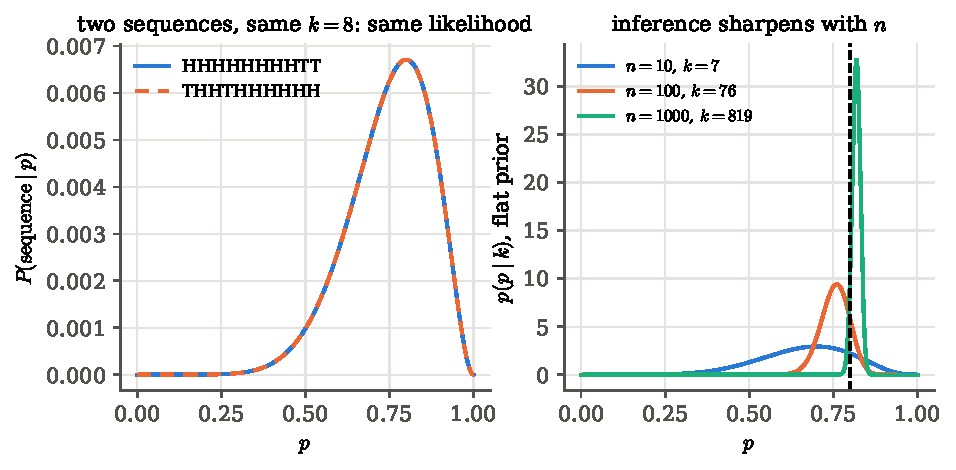
\includegraphics[width=\linewidth]{figures/ch00/pipeline_coin.pdf}
\caption{Left: the likelihoods of two different toss sequences with the same
number of heads lie exactly on top of each other, so the summary $k$ lost
nothing. Right: the flat-prior posterior for $p$ after 10, 100 and 1000
tosses of one coin with true $p=0.8$ (dashed line). The width shrinks like
$1/\sqrt n$.}
\label{0a:fig:pipeline-coin}
\end{figure}

\paragraph{How research uses the pipeline.}
In current research the hard stages are the middle ones. For the coin and the
full-sky Gaussian CMB every stage has a closed form, but real problems rarely
do. Which summary of a galaxy survey carries the neutrino mass: the power
spectrum $P(k)$, the bispectrum, void counts, Betti numbers? What is
$P(S\given\params)$ when $S$ is measured on a masked, noisy, nonlinear field?
Usually nobody can write it down. So one simulates the forward model many
times at fixed $\params$ and estimates the mean and covariance of $S$ from the
simulations (\cref{ch:08,ch:12}). The inference stage then uses the standard
machinery of \cref{ch:05,ch:09,ch:10}.

\begin{pitfall}[the posterior depends on the summary]
If $S$ is not sufficient, $P(\params\given S)$ is broader than
$P(\params\given\data)$, and it can be broader in a direction that matters. That
is not a bug of Bayes' theorem; it is the price of the compression chosen at
stage~4. Two analyses of the same data with different summaries can
legitimately give different constraints.
\end{pitfall}

\paragraph{Kruschke's five steps.}
The pipeline is the physicist's version of the five steps of Bayesian data
analysis \srcref{Kruschke}{p.~25}. They match the six stages one by one.
\emph{Identify the data relevant to the research question}: stages 2 and 3,
the dataset and the choice of what information matters. \emph{Define a
descriptive model for the data}: stages 1 and 5, the model and the sampling
distribution. \emph{Specify a prior}: the factor $P(\params)$ of stage 6.
\emph{Reallocate credibility across parameter values}: the posterior of
stage 6. \emph{Check the posterior predictions}: the dashed loop of
\cref{0a:fig:pipeline}.

\section{Which summary? From amplitude to topology}\label{0a:sec:summaries}

Two simulated universes are handed to us as density maps. In one, the dense
matter forms a connected web of filaments. In the other, it sits in isolated
clumps. By construction both maps have the same mean, the same variance and
the same power spectrum $P(k)$. An analysis that compresses each map to $P(k)$
will call them identical, yet a glance tells them apart.

Whether we catch this difference or miss it is decided at the third stage of
the pipeline of \cref{0a:sec:pipeline}: \emph{deciding which features carry
the physics}. The power spectrum answers one question: how much variance does
each scale carry? The two maps raise a different one. Is there physically
meaningful information in the way the high and low regions of a field are
connected, information that the summary we already use, here $P(k)$, does not
bring out? A field admits several kinds of summary, and two fields can be
built to agree on some kinds and differ on the others. Topological summaries
are worth the trouble for a second reason too: some of them are protected
against the distortions that observation introduces.

\paragraph{A recording with its phases scrambled.}
Take a recording of speech, $h(t)$, and Fourier transform it to $\tilde h(f)$.
Keep every amplitude $|\tilde h(f)|$ and replace every phase by a random one.
The power spectrum is untouched, and so is the loudness, yet the result is a
hiss. What made it speech was in the phases: in \emph{where} and \emph{how}
the power is arranged in time. For a field, the phases decide whether high
values line up into filaments, gather into blobs or scatter as noise.
Summaries beyond the power spectrum are ways of reading the phases.

\paragraph{The central question for a field.}
A theory predicts a field $\phi(\mathbf x)$ over space. The experiment gives
us one copy of it, and an imperfect one. On the way to us its values have been
pushed around by perturbations, by noise, by smoothing, by whatever happened
to the signal while it travelled. The question is whether something about the
\emph{shape and structure} of what we receive survives every change we count
as a nuisance. If it does, we can read it off without first undoing those
changes. Write such a change as a \newterm{nuisance transformation}
$\phi\to\phi'=\mathcal N[\phi]$; examples are noise, smoothing by a beam,
lensing, and a monotonic response of the detector. Three questions follow.
\begin{enumerate}[leftmargin=2em]
  \item What do we want to know: how large the field is, how its values at different points are related, or how its structures are shaped and connected?
  \item Which summary $T$ answers that question?
  \item Is there a summary that the nuisance cannot change, $T[\mathcal N[\phi]]=T[\phi]$, for a stated class of $\mathcal N$?
\end{enumerate}

The answers to the first question form a ladder. Each rung up keeps less of
the raw values and more of how they are arranged.

\begin{taxonomy}[the summaries of a field]
\small
\renewcommand{\arraystretch}{1.3}
\begin{tabularx}{\linewidth}{@{}>{\raggedright\arraybackslash}p{2.3cm}
  >{\raggedright\arraybackslash}X >{\raggedright\arraybackslash}p{4.4cm}@{}}
\toprule
\textbf{kind} & \textbf{the question it answers} & \textbf{examples}\\
\midrule
amplitude & how large is the field typically? & $\langle\phi\rangle$, $\Var(\phi)$, the one-point pdf $P(\phi)$\\
correlation & how are values a distance $r$ apart related? & $\xi(r)$, $P(k)$, $\Cell$\\
higher order & is there information beyond Gaussian two-point statistics? & bispectrum $B$, trispectrum $T$, skewness\\
morphology & what sizes and shapes do the structures have? & areas, perimeters, curvature of excursion sets\\
topology & how are the structures connected, and how many holes do they have? & Betti numbers $\beta_i$, Euler characteristic $\chi$, persistence\\
\bottomrule
\end{tabularx}
\smallskip
These are not rival theories of probability. They are different maps from
the same data to different summaries $S[\phi]$. Once $S$ is chosen it is an
ordinary random observable with a sampling distribution $P(S\given\params)$,
and \cref{ch:03,ch:04,ch:05,ch:09,ch:10} apply to it unchanged.
\end{taxonomy}

A \emph{Gaussian} random field is special: all its information is in the
first two rungs. Its higher-order summaries are fixed functions of its power
spectrum. Measuring them is therefore a consistency test (a search for
non-Gaussianity), not new information. For any non-Gaussian field, from the
late-time cosmic web to a map with foreground residuals, the upper rungs carry
information that $P(k)$ does not.

Topology is a property of shapes, not of functions. So to say what topology
measures, we must first turn a field into a shape.

\begin{workdef}[excursion set, Betti numbers, Euler characteristic]
For a threshold $\nu$, the \newterm{excursion set} of $\phi$ on a domain
$\mathcal M$ is
\begin{equation}
  X_\nu=\{\mathbf x\in\mathcal M:\ \phi(\mathbf x)>\nu\}
  \label{0a:eq:excursion}
\end{equation}
\unpack{the region of the map where the field exceeds $\nu$, e.g.\ the sky
directions hotter than $\nu$}. In two dimensions the \newterm{Betti numbers}
are $\beta_0(X_\nu)$ \unpack{the number of separate pieces} and $\beta_1(X_\nu)$
\unpack{the number of independent holes, i.e.\ enclosed regions that are not part of the set}. The
\newterm{Euler characteristic} is $\chi=\beta_0-\beta_1$. These numbers do
not change when the set is stretched or bent without tearing or gluing
(\cref{ch:12}). A summary $T$ is a \newterm{robust observable} under a
class of nuisance transformations if $T[\mathcal N[\phi]]=T[\phi]$ for every
$\mathcal N$ in the class.
\end{workdef}

\begin{figure}[htbp]
\centering
\begin{tikzpicture}
  \begin{scope}[x=0.55cm,y=0.75cm]
    \draw[->,softgray] (0.4,-1.7) -- (10.3,-1.7) node[anchor=north east,font=\footnotesize] {$x$};
    \draw[->,softgray] (0.6,-1.7) -- (0.6,2.1) node[anchor=east,font=\footnotesize] {$\phi$};
    \draw[form] plot[domain=0.6:10,samples=160,smooth]
      (\x,{0.9*sin(1.1*\x r)+0.55*sin((2.7*\x+1.0) r)+0.3*cos((4.3*\x+0.5) r)});
    \begin{scope}
      \clip (0.6,0.6) rectangle (10,2.0);
      \draw[bdry] plot[domain=0.6:10,samples=160,smooth]
        (\x,{0.9*sin(1.1*\x r)+0.55*sin((2.7*\x+1.0) r)+0.3*cos((4.3*\x+0.5) r)});
    \end{scope}
    \draw[dashed,black] (0.6,0.6) -- (10,0.6);
    \node[font=\footnotesize,anchor=west] at (10,0.6) {$\nu$};
    \foreach \a/\b in {1.133/1.534,2.129/2.877,6.641/7.723}
      {\draw[bdryred,line width=2.2pt] (\a,-1.7) -- (\b,-1.7);}
    \node[font=\footnotesize,bdryred,anchor=north] at (5.3,-1.9) {$X_\nu$: three pieces, $\beta_0=3$};
  \end{scope}
  \begin{scope}[xshift=7.1cm,yshift=0.3cm]
    \fill[bdryred!55] (0,0.9) circle (0.42);
    \node[font=\scriptsize,align=center,anchor=north] at (0,0.35) {$\beta_0{=}1,\ \beta_1{=}0$\\$\chi=1$};
    \fill[bdryred!55,even odd rule] (1.9,0.9) circle (0.45) (1.9,0.9) circle (0.2);
    \node[font=\scriptsize,align=center,anchor=north] at (1.9,0.35) {$\beta_0{=}1,\ \beta_1{=}1$\\$\chi=0$};
    \fill[bdryred!55] (-0.2,-0.9) circle (0.25) (0.3,-0.75) circle (0.2);
    \node[font=\scriptsize,align=center,anchor=north] at (0.05,-1.3) {$\beta_0{=}2,\ \beta_1{=}0$\\$\chi=2$};
    \fill[bdryred!55,even odd rule] (1.9,-0.85) ellipse (0.6 and 0.38)
      (1.65,-0.85) circle (0.13) (2.15,-0.85) circle (0.13);
    \node[font=\scriptsize,align=center,anchor=north] at (1.9,-1.3) {$\beta_0{=}1,\ \beta_1{=}2$\\$\chi=-1$};
  \end{scope}
\end{tikzpicture}
\caption{Left: a field along a line, a threshold $\nu$, and the excursion set
(the red intervals on the axis), which here has three pieces. Right: four
two-dimensional sets with their numbers of pieces $\beta_0$, holes $\beta_1$
and Euler characteristic $\chi=\beta_0-\beta_1$. Stretching any of them leaves
all three numbers unchanged; cutting or gluing does not.}
\label{0a:fig:excursion}
\end{figure}

Two facts make these summaries useful. First, a change of phases can leave the
lower rungs untouched while moving the upper ones. Second, a distortion that
changes each value by the same increasing function leaves the excursion sets
themselves untouched. Each takes a few lines to prove.

\zeroaEx{phase randomisation keeps the power spectrum and the variance}
\label{0a:ex:phases}
The question: if we keep every Fourier amplitude of a field and scramble the
phases, what stays the same? Let $\phi(\mathbf x)$ live on an $N$-pixel
periodic grid with zero mean, and let
$\tilde\phi_{\mathbf k}=\sum_{\mathbf x}\phi(\mathbf x)e^{-2\pi i\mathbf k\cdot\mathbf x/L}$
be its discrete Fourier transform ($L$ the side length in pixels). Build a new
field $\phi'$ with $\tilde\phi'_{\mathbf k}=|\tilde\phi_{\mathbf k}|e^{i\alpha_{\mathbf k}}$,
random phases $\alpha_{\mathbf k}$ with $\alpha_{-\mathbf k}=-\alpha_{\mathbf k}$
(so that $\phi'$ is real). Then
\begin{align*}
  P'(k) &\eqby{1} \big\langle|\tilde\phi'_{\mathbf k}|^2\big\rangle_{|\mathbf k|=k}
   \eqby{2} \big\langle|\tilde\phi_{\mathbf k}|^2\big\rangle_{|\mathbf k|=k}=P(k),\\
  \Var(\phi') &\eqby{3} \frac1N\sum_{\mathbf x}\phi'(\mathbf x)^2
   \eqby{4} \frac1{N^2}\sum_{\mathbf k}|\tilde\phi'_{\mathbf k}|^2
   \eqby{5} \frac1{N^2}\sum_{\mathbf k}|\tilde\phi_{\mathbf k}|^2
   = \Var(\phi) .
\end{align*}
\begin{explain}
  \item The measured power spectrum: average $|\tilde\phi_{\mathbf k}|^2$ over the wavevectors in a shell of radius $k$.
  \item $|re^{i\alpha}|^2=r^2$: the phase drops out of every $|\tilde\phi'_{\mathbf k}|^2$ individually.
  \item Zero mean (the $\mathbf k=0$ coefficient, the sum of the field, is left at zero).
  \item Parseval's theorem for the discrete Fourier transform, $\sum_{\mathbf x}|\phi(\mathbf x)|^2=\frac1N\sum_{\mathbf k}|\tilde\phi_{\mathbf k}|^2$.
  \item Same step as (2).
\end{explain}
So every summary built from the amplitudes $|\tilde\phi_{\mathbf k}|$ alone is
identical for $\phi$ and $\phi'$. The skewness, the excursion sets and their
Betti numbers depend on the phases, so they are free to change.

\zeroaEx{a monotonic distortion leaves the excursion sets alone}
\label{0a:ex:monotonic}
Suppose the detector does not record $\phi$ itself but
$\phi'(\mathbf x)=f(\phi(\mathbf x))$, with $f$ strictly increasing. Examples are a detector
with a nonlinear but monotonic response, or a lognormal model $\phi'=e^{\phi}$.
The question: which summaries of $\phi$ can we still read off $\phi'$ without
knowing $f$? Compare the excursion sets. For every threshold $\nu$
\begin{align*}
  X'_{f(\nu)} &\eqby{1} \{\mathbf x:\ f(\phi(\mathbf x))>f(\nu)\}
   \eqby{2} \{\mathbf x:\ \phi(\mathbf x)>\nu\} = X_\nu .
\end{align*}
\begin{explain}
  \item Definition \eqref{0a:eq:excursion} applied to $\phi'$ at the threshold $f(\nu)$.
  \item A strictly increasing $f$ preserves order both ways: $f(a)>f(b)$ exactly when $a>b$.
\end{explain}
The excursion sets are the same regions of the domain $\mathcal M$. So the
curves $\beta_0(\nu)$, $\beta_1(\nu)$, $\chi(\nu)$ are the same, except that
the threshold is relabelled $\nu\to f(\nu)$. Meanwhile the variance, the
skewness and $P(k)$ of $\phi'$ all change; for $f=\exp$ the one-point pdf goes
from Gaussian to lognormal. Here topology is a robust observable in the exact
sense of the working definition above, $T[\mathcal N[\phi]]=T[\phi]$; the power
spectrum is not.

\zeroaEx{counting holes by counting cells}
\label{0a:ex:cells}
How do we count holes in a real map, where nobody can look at every piece?
On a pixel grid a set is a union of square pixels, and $\chi$ can be computed
by counting: $\chi=V-E+F$. Here $V$ is the number of corners, $E$ the number of
pixel edges and $F$ the number of pixels of the set, each counted once. A
single pixel has $4-4+1=1$. Two separate pixels have $8-8+2=2$. Now take a
ring of eight pixels around an empty centre (a $3\times3$ block with the
middle removed). It uses all $4\times4=16$ corners of the block, $12$
horizontal and $12$ vertical edges, and $8$ pixels:
\[
  \chi=16-24+8=0=\beta_0-\beta_1=1-1 .
\]
So local counting finds a hole without ever looking for it. That is how
$\chi(\nu)$ is computed on real maps (\cref{ch:12}).

\paragraph{What this bought us.}
The ladder of summaries is a ladder of questions. Two fields can agree on the
bottom two rungs and differ above them. And some topological summaries are
exactly unchanged by a class of distortions that change every rung below.

\subsection*{Two fields with one power spectrum}

The script \pyname{04_same_spectrum.py} builds the two universes from the
opening of \cref{0a:sec:summaries}: one clumpy, one not, with the same power
spectrum. Field A drops $\SameNblob$ points at random on a $256\times256$
periodic grid and smooths them into blobs. Field B is A with its phases
randomised, exactly as in \cref{0a:ex:phases}:

\pyfile[firstline=28,lastline=34]{code/ch00/04_same_spectrum.py}{Keeping every $|\tilde\phi_k|$ and replacing the phases}

The random phases are taken from the Fourier transform of a real white-noise
map. Such phases automatically satisfy the condition
$\alpha_{-\mathbf k}=-\alpha_{\mathbf k}$, so B is real. Pieces are counted
with the function \pyname{scipy.ndimage.label}, which labels connected groups
of pixels above the threshold.

The run shows the lower rungs agreeing and the upper ones not. The variances
are $\Var(A)=\SameVarA$ and $\Var(B)=\SameVarB$, and the two binned power
spectra differ by at most a fraction $\SamePkMaxDev$, which is round-off. The
skewness separates the fields: $\SameSkewA$ for the clumps of A, $\SameSkewB$
for B, which is close to Gaussian. The topology separates them more sharply.
At $\nu=3$ (three standard deviations) A has $\beta_0=\SameBzeroA$ separate
pieces, one per surviving blob, and B has $\SameBzeroB$. At $\nu=0$ the counts
are $\SameBzeroAzero$ and $\SameBzeroBzero$.

\begin{figure}[htbp]
\centering
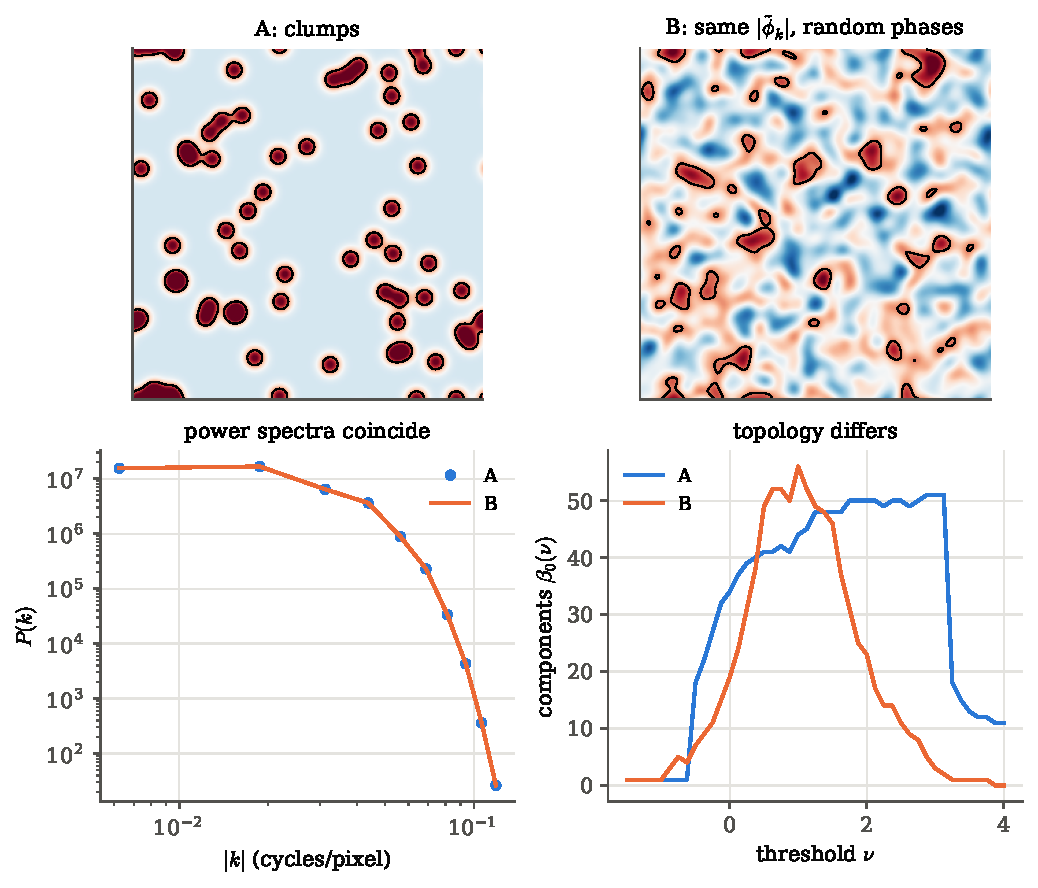
\includegraphics[width=0.92\linewidth]{figures/ch00/same_spectrum.pdf}
\caption{Top: the clumpy field A and its phase-randomised twin B, with the
contour at $\nu=1.5$. Bottom left: their power spectra coincide point by point.
Bottom right: the number of connected pieces of the excursion set as the
threshold is raised. B behaves like a Gaussian field, with most pieces near
$\nu\approx1$ and few at high threshold; A keeps one piece per blob right up to
the blob peaks, so its curve stays high until $\nu\approx3$.}
\label{0a:fig:same-spectrum}
\end{figure}

\subsection*{Topology that survives observation, and topology that records dynamics}

The detector with a monotonic response (\cref{0a:ex:monotonic}) is the
simplest protected case. A more physical one is CMB polarisation. The linear
polarisation is described by the two Stokes parameters $Q$ and $U$, which
combine into $P=Q+iU$. At isolated points where $Q=U=0$ the polarisation
direction is undefined. Walk once round such a \newterm{polarisation
singularity}, and the phase of $P$ turns by a whole multiple of $2\pi$. This
whole number, the winding index or charge, cannot change under a smooth
one-to-one remapping of the sky such as weak lensing. Lensing certainly
changes the polarisation map, converting $E$ modes into $B$ modes. But it can
only move and distort singularities; it cannot change their charges
continuously \cite{VachaspatiLue2003,HutererVachaspati2005,ChallinorChon2002}.
The protection fails where its assumptions fail: pairs of singularities can be
created or annihilated, and noise and finite resolution can hide them.

A count at a single threshold is fragile, since nothing makes $\nu=1\sigma$
special. The remedy is to follow each piece and hole as $\nu$ is lowered.
Record the threshold where each feature appears (its birth) and the one where
it merges or fills in (its death). This gives \newterm{persistence}. A feature
with a long lifetime $\Delta\nu=\nu_{\rm death}-\nu_{\rm birth}$ is a real
structure; a short-lived one is likely noise. \Cref{ch:12} builds this with a
union--find algorithm.

\begin{pitfall}[topology is not conserved by dynamics]
Invariance holds under a stated class of deformations, not under physics in
general. Gravitational collapse is not a monotonic remapping of the initial
density: it moves matter, merges clumps and opens voids, and the Betti numbers
of the cosmic web change with time \cite{Wilding2021,Pranav2017}. There the
changing topology is the \emph{signal}. The scientific question is either
``what survives the nuisance?'' or ``what changes because of the physics?''.
Both are legitimate; they are different questions. Note also that a mask cuts
excursion sets at its edge and so changes their topology, just as it changes
the covariance of $\Chat$ (\cref{ch:08}).
\end{pitfall}

\paragraph{How research uses a topological summary.}
A CMB map is a function $T:S^2\to\R$ from directions on the sphere to
temperatures. To use its topology, generate many Gaussian skies from the
fiducial power spectrum $\Cell$. Pass each sky through the beam, the noise and
the mask. Measure $\beta_0(\nu)$, $\beta_1(\nu)$ and $\chi(\nu)$ on every
realisation. The mean and covariance of these curves over the realisations
define a likelihood for the observed curves, and the posterior follows as for
any other summary. This is the Monte Carlo study of \cref{ch:08} with $\Chat$
replaced by a Betti curve, and it is where the book ends (\cref{ch:12}).

\section{One idea, several detectors}\label{0a:sec:universal}

A collider experiment counts events in bins of invariant mass and asks whether
there is a bump. A CMB satellite measures the temperature of the sky and asks
for the cosmological parameters. A gravitational-wave interferometer records a
strain time series and asks for the masses of an inspiralling binary. The
instruments share nothing, and the statistics looks different in each
community's papers: Poisson log-likelihoods, $\Cell$ likelihoods, matched
filters. Underneath, all three ask one question: \emph{for a given set of
parameters $\params$, how probable is the noise realisation that would turn
the model's prediction into the data we actually recorded?} Because the
question is the same, the idea needs to be developed only once. Writing it out
for each detector, and for a topological summary, shows how it applies
everywhere.

\paragraph{The noise you would need.}
The likelihood is the probability density of the noise that the data
require. Put the model prediction $m(\params)$ on one side and the data
$\data$ on the other. The difference $\data-m(\params)$ is the noise that
nature \emph{would have had to supply} if $\params$ were the truth. A value of
$\params$ that needs a wildly improbable noise realisation is implausible. A
value that needs only a typical fluctuation is plausible. What differs between
detectors is only the statistics of their noise. \Cref{ch:03} builds the
likelihood from this picture one step at a time.

\paragraph{The same four questions for any detector.}
\begin{enumerate}[leftmargin=2em]
  \item What does the model predict, as a function of $\params$?
  \item What is the noise: its distribution, and its correlations?
  \item For a trial $\params$, how probable is the noise realisation $\data-m(\params)$ (or, for counts, the observed counts given their expectation)?
  \item Read that probability as a function of $\params$, and feed it to Bayes, MCMC or Fisher.
\end{enumerate}

\begin{workdef}[likelihood from a noise model]
If the data are prediction plus noise, $\data=m(\params)+\bm\epsilon$, and the
noise has a known density $p_\epsilon$, then
\begin{equation}
  \Like(\params)\equiv p(\data\given\params)=p_\epsilon\big(\data-m(\params)\big)
  \label{0a:eq:like-noise}
\end{equation}
\unpack{the density of the noise realisation that is required, evaluated at
the observed data and read as a function of $\params$}. The
\newterm{likelihood} is not a probability distribution over $\params$: it need
not integrate to one over $\params$, and only its shape and ratios matter.
\end{workdef}

\begin{figure}[htbp]
\centering
\begin{tikzpicture}[x=1.05cm,y=1.1cm]
  \draw[->,softgray] (0,0) -- (8.6,0) node[anchor=north east,font=\footnotesize] {$x$};
  \draw[->,softgray] (0,0) -- (0,4.1) node[anchor=east,font=\footnotesize] {$d$};
  \draw[form] (0.3,0.905) -- (8.2,3.67);
  \node[font=\footnotesize,formblue,anchor=west] at (8.2,3.67) {$m(x;\theta)$};
  \foreach \x/\r in {1/0.35,2/-0.30,3/0.15,4/-0.55,5/0.25,6/0.45,7/-0.20}{
    \pgfmathsetmacro{\m}{0.8+0.35*\x}
    \draw[bdryred,thick] (\x,\m) -- (\x,{\m+\r});
    \fill[black] (\x,{\m+\r}) circle (1.6pt);
  }
  \draw[fibre] plot[domain=-1.1:1.1,samples=50,smooth]
    ({4+0.9*exp(-(\x)^2/(2*0.35^2))},{2.2+\x});
  \draw[faint] (4,1.1) -- (4,3.3);
  \node[font=\footnotesize,fibreorange,anchor=west,align=left] at (5.05,1.25) {$p(d_4\given\theta)$: how probable\\ is the red residual?};
  \node[font=\footnotesize,bdryred,anchor=east,align=right] at (3.85,0.45) {required noise\\ $\epsilon_i=d_i-m(x_i;\theta)$};
\end{tikzpicture}
\caption{Data as prediction plus noise. The blue line is the model for one
trial value of $\theta$; the black points are the data; the red segments are
the noise each point would need if that $\theta$ were true. The orange curve
at the fourth point is the Gaussian noise density: a long red segment lands in
its tail and costs a lot of probability. The likelihood multiplies these costs
over all points; moving $\theta$ moves the line and changes every red segment.}
\label{0a:fig:residuals}
\end{figure}

The commonest case is independent Gaussian noise: each data point $d_i$ has
its own noise $\epsilon_i\sim\Normal(0,\sigma_i^2)$, a Gaussian with mean zero
and standard deviation $\sigma_i$. Then \eqref{0a:eq:like-noise} gives the
workhorse of physics:
\begin{align}
  \ln\Like(\params)
  &\eqby{1} \ln\prod_{i=1}^{N}\frac{1}{\sqrt{2\pi\sigma_i^2}}
    \exp\!\Big[-\frac{(d_i-m_i(\params))^2}{2\sigma_i^2}\Big] \nonumber\\
  &\eqby{2} -\frac12\sum_{i=1}^{N}\frac{(d_i-m_i(\params))^2}{\sigma_i^2}
    -\frac12\sum_{i=1}^{N}\ln(2\pi\sigma_i^2)
   \equiv -\frac12\chi^2(\params)+\text{const} .
  \label{0a:eq:chi2}
\end{align}
\begin{explain}
  \item Independent noise: the joint density is the product of one Gaussian per data point, evaluated at the required noise $d_i-m_i(\params)$.
  \item The log of a product is the sum of logs, and $\ln e^{u}=u$.
\end{explain}
If the noise in different data points is correlated, with covariance matrix
$\Cmat$, the product of separate Gaussians becomes one multivariate Gaussian:
$\ln\Like=-\frac12(\data-m)\T\Cmat^{-1}(\data-m)-\frac12\ln\det(2\pi\Cmat)$.
The statistical logic is the same as before. Only the model for the
probability of the data has changed.

With a whole data vector and many parameters, the backward question of
\cref{0a:sec:two-directions} is still the same. The data vector is what we
saw. Every value of $\params$ is a candidate explanation. The likelihood says
how readily each candidate would have produced those data (\cref{ch:05}).
Reading the likelihood as the plausibility of the fluctuation needed to turn
the model into the data is also how maximum likelihood is motivated
\mainref{p.~122}.

\begin{taxonomy}[one question, four implementations]
\small
\renewcommand{\arraystretch}{1.3}
\begin{tabularx}{\linewidth}{@{}>{\raggedright\arraybackslash}p{1.9cm}
  >{\raggedright\arraybackslash}p{2.4cm} >{\raggedright\arraybackslash}X
  >{\raggedright\arraybackslash}p{4.1cm}@{}}
\toprule
\textbf{experiment} & \textbf{data} & \textbf{noise model} & \textbf{log-likelihood}\\
\midrule
collider & counts $n_i$ in bins & Poisson with mean $\lambda_i(\mu)=b_i+\mu s_i$ & $\sum_i[n_i\ln\lambda_i-\lambda_i]$\\
CMB & $\alm$, or $\Chat$ & Gaussian random field on the sphere, variance $\Cell$ per mode & $-\frac12\sum_\ell(2\ell+1)\big[\Chat/\Cell+\ln\Cell\big]$\\
GW detector & strain $d(t)$ & stationary Gaussian noise with PSD $S_n(f)$ & $-\frac12(d-h\,|\,d-h)$\\
topology & Betti curves $S=\beta_0(\nu),\dots$ & unknown in closed form: simulated & $-\frac12(S-\bar S)\T\widehat{\Cmat}^{-1}(S-\bar S)$ from simulations\\
\bottomrule
\end{tabularx}
\end{taxonomy}

\zeroaEx{the collider: a bump in Poisson counts}
\label{0a:ex:poisson}
The data are event counts $n_i$ in bins $i$ of invariant mass. The question:
how probable are these counts for a given signal strength $\mu$? In bin $i$
the expected count is $\lambda_i(\mu)=b_i+\mu s_i$: the background $b_i$ plus a
signal template $s_i$ scaled by $\mu$. Counts in different bins are
independent Poisson variables. Then
\begin{align*}
  \ln\Like(\mu)
  &\eqby{1} \ln\prod_i\frac{\lambda_i^{n_i}e^{-\lambda_i}}{n_i!}
   \eqby{2} \sum_i\big[n_i\ln\lambda_i(\mu)-\lambda_i(\mu)\big]-\sum_i\ln n_i!,\\
  \frac{\dd\ln\Like}{\dd\mu}
  &\eqby{3} \sum_i s_i\Big(\frac{n_i}{\lambda_i(\mu)}-1\Big)=0
  \quad\text{at the maximum-likelihood }\hat\mu .
\end{align*}
\begin{explain}
  \item Poisson probability of $n_i$ events when $\lambda_i$ are expected (\cref{ch:02}), multiplied over independent bins.
  \item Log of a product; the last sum does not depend on $\mu$ and drops out of every ratio.
  \item $\dd\lambda_i/\dd\mu=s_i$; the chain rule on $n_i\ln\lambda_i$ gives $n_is_i/\lambda_i$.
\end{explain}
The condition says that at the best fit the observed counts match the
expected ones on average, with each bin weighted by its signal $s_i$. There is
no $\sigma_i$ anywhere. The Poisson distribution carries its own noise: its
variance equals its mean.

\zeroaEx{the CMB: the full-sky $\Cell$ likelihood}
\label{0a:ex:cmb-like}
The data are the harmonic coefficients of the sky (\cref{0a:ex:cmb-pipeline});
the parameters are the power spectrum values $\Cell$. The question: how
probable is the observed sky for given $\Cell$? Write the sky in a real
orthonormal basis of spherical harmonics, so that at each multipole $\ell$
there are $2\ell+1$ real coefficients $r_{\ell j}$. For a Gaussian isotropic
sky they are independent, and each is $\Normal(0,\Cell)$. Then
\begin{align*}
  \ln\Like(\{\Cell\})
  &\eqby{1} \sum_{\ell}\sum_{j=1}^{2\ell+1}\Big[-\frac{r_{\ell j}^2}{2\Cell}-\frac12\ln(2\pi\Cell)\Big]\\
  &\eqby{2} -\frac12\sum_\ell\Big[\frac{(2\ell+1)\Chat}{\Cell}+(2\ell+1)\ln\Cell\Big]+\text{const}\\
  &= -\frac12\sum_\ell(2\ell+1)\Big[\frac{\Chat}{\Cell}+\ln\Cell\Big]+\text{const}.
\end{align*}
\begin{explain}
  \item \eqref{0a:eq:chi2} with $d_i\to r_{\ell j}$, zero mean and variance $\Cell$.
  \item $\sum_j r_{\ell j}^2=(2\ell+1)\Chat$, the definition of $\Chat$ in \cref{0a:ex:cmb-pipeline} (a real orthonormal basis is a rotation of the complex one, so the sum of squares is unchanged); $\ln 2\pi$ goes into the constant.
\end{explain}
Three things follow. First, the data enter only through $\Chat$, so $\Chat$
is sufficient in the sense of \eqref{0a:eq:factorisation}, as claimed in
\cref{0a:ex:cmb-pipeline}. Second, setting
$\partial\ln\Like/\partial\Cell=\frac12(2\ell+1)[\Chat/\Cell^2-1/\Cell]=0$
gives $\Cell=\Chat$: the measured spectrum is the best fit. Third,
$(2\ell+1)\Chat/\Cell=\sum_j(r_{\ell j}/\sqrt{\Cell})^2$ is a sum of $2\ell+1$
squared unit Gaussians, which is a $\chi^2_{2\ell+1}$ variable (\cref{ch:02}).
That is how the script below simulates one sky's spectrum without making a
map.

\zeroaEx{the GW detector: Gaussian noise with a PSD}
\label{0a:ex:whittle}
The detector records a strain $d(t)=h(t;\params)+n(t)$ for a time $T$: a
signal $h$ from the binary with parameters $\params$, plus noise $n$. The
question: how probable is the required noise $d-h$ for given $\params$? The
noise is simplest in frequency space, so Fourier transform,
$\tilde d(f)=\int d(t)e^{-2\pi ift}\dd t$, at the frequencies $f_k=k/T$, and
write $\tilde d_k=\tilde d(f_k)$. Stationary Gaussian noise has independent
Fourier modes. Its one-sided power spectral density $S_n(f)$ \unpack{the
noise power per unit frequency, counting positive frequencies only} fixes
their size, $\E|\tilde n_k|^2=\frac T2 S_n(f_k)$. We also need one fact about
complex Gaussians. A complex Gaussian $z$ with $\E|z|^2=\sigma^2$ has density
$\frac{1}{\pi\sigma^2}e^{-|z|^2/\sigma^2}$ (its real and imaginary parts are
independent, each with variance $\sigma^2/2$). So
\begin{align*}
  \ln\Like(\params)
  &\eqby{1} -\sum_{k}\frac{|\tilde d_k-\tilde h_k(\params)|^2}{\tfrac T2 S_n(f_k)}+\text{const}
   \eqby{2} -2\sum_k\Delta f\,\frac{|\tilde d_k-\tilde h_k|^2}{S_n(f_k)}+\text{const}\\
  &\eqby{3} -2\int_0^\infty\frac{|\tilde d(f)-\tilde h(f)|^2}{S_n(f)}\,\dd f+\text{const}
   \eqby{4} -\frac12\,(d-h\,|\,d-h)+\text{const},
\end{align*}
\begin{explain}
  \item The required noise in mode $k$ is $\tilde d_k-\tilde h_k$; the product of independent complex Gaussians becomes a sum in the log. The $-\ln(\pi\sigma^2)$ terms do not depend on $\params$.
  \item The mode spacing is $\Delta f=1/T$, so $\frac{1}{T/2}=2\Delta f$.
  \item For long $T$ the sum over modes becomes an integral over positive frequencies.
  \item Definition of the noise-weighted inner product $(a\,|\,b)=4\,\mathrm{Re}\int_0^\infty\tilde a(f)\tilde b^*(f)/S_n(f)\,\dd f$.
\end{explain}
This is the $\chi^2$ of \eqref{0a:eq:chi2} in the frequency domain, with each
frequency weighted by how noisy the detector is there. Maximising it over
$\params$ is matched filtering. Its curvature gives the Fisher matrix of
\cref{ch:10}.

\paragraph{What this bought us.}
Poisson counts, a Gaussian sky and coloured detector noise give three
formulas that look unrelated. Each one is \eqref{0a:eq:like-noise}: the
probability of the fluctuation that would turn the prediction into the data.

\subsection*{The three detectors in code}

The script \pyname{05_three_detectors.py} generates data for all three and
checks the noise model of each. For the collider and the GW detector the key lines are:

\pyfile[firstline=27,lastline=33]{code/ch00/05_three_detectors.py}{Collider: Poisson data and a scan of $\ln\Like(\mu)$}
\pyfile[firstline=53,lastline=58]{code/ch00/05_three_detectors.py}{GW: coloured Gaussian noise drawn in the frequency domain}

\emph{Collider.} The first block draws one Poisson count per bin. The
expected counts are a falling background plus a peak at $125$ GeV with
$\mu=1$. It then evaluates the $\ln\Like$ of \cref{0a:ex:poisson} on a grid of
$\mu$. With $\ColNtot$ events in total, the maximum is at
$\hat\mu=\ColMuHat$. The values of $\mu$ whose $\ln\Like$ lies within
$\frac12$ of the maximum run from $\ColMuLo$ to $\ColMuHi$; for a nearly
Gaussian likelihood this is the $\pm1\sigma$ interval (\cref{ch:03}). The true
$\mu=1$ is inside.

\emph{GW detector.} The second block draws each Fourier mode with real and
imaginary parts of variance $TS_n/4$, so that $\E|\tilde n_k|^2=TS_n/2$. The
periodogram $2|\tilde d_k|^2/T$ should then scatter around $S_n$. Averaged
over $\GwNbins$ frequency bins away from the injected line, its ratio to $S_n$
is $\GwMeanRatio$.

\emph{CMB.} One full sky is simulated as
$\Chat=\Cell\,\chi^2_{2\ell+1}/(2\ell+1)$ around the Planck best fit, using
the third result of \cref{0a:ex:cmb-like}. The mean of $\Chat/\Cell$ over
$2\le\ell\le1500$ is $\CmbMeanRatio$. Its scatter is $\CmbScatterLow$ for
$\ell\le30$ but only $\CmbScatterHigh$ for $\ell>1000$, as the cosmic-variance
formula $\sqrt{2/(2\ell+1)}$ predicts.

\begin{figure}[htbp]
\centering
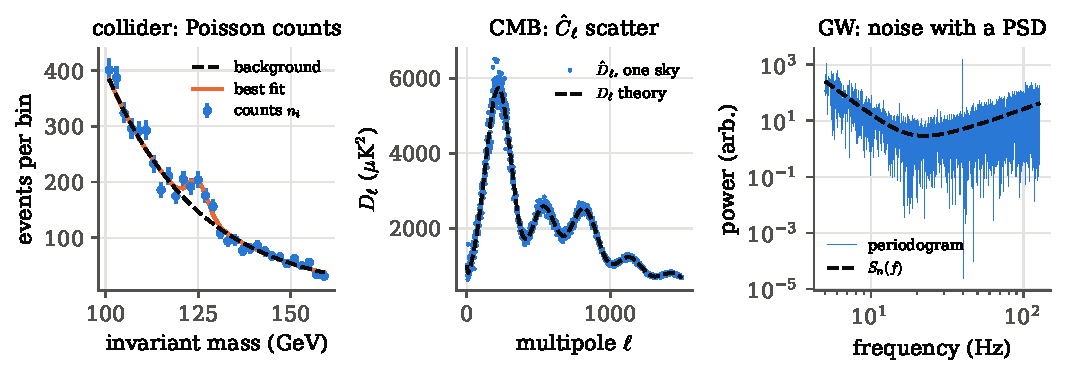
\includegraphics[width=\linewidth]{figures/ch00/three_detectors.pdf}
\caption{The same logic in three instruments. Left: Poisson counts with
$\sqrt{n}$ error bars over a falling background, and the best-fit background
plus signal. Middle: one simulated sky's $\hat D_\ell$ scattering around the
theory curve; the scatter is large at low $\ell$, where there are few modes,
and small at high $\ell$. Right: the periodogram of simulated detector noise,
wildly fluctuating from bin to bin but centred on the power spectral density.}
\label{0a:fig:three-detectors}
\end{figure}

\paragraph{How research uses these likelihoods.}
Each simulation here verifies a known noise model: Poisson counts, $\chi^2$
scatter of $\Chat$, a periodogram centred on $S_n$. In research the closed
forms break. A galactic mask couples multipoles and makes the $\Cell$
likelihood non-diagonal. Real interferometer noise has glitches and is not
stationary. A Betti curve has no known distribution at all. The fix is always
the fourth row of the taxonomy (topology): simulate the forward model,
estimate the mean and covariance of the summary from the simulations, and use
the Gaussian form. The price is that the estimated covariance
$\widehat{\Cmat}$ is itself noisy and must be corrected \cite{Hartlap2007}
(\cref{ch:08}).

\begin{pitfall}[the likelihood is not the posterior]
$\Like(\params)=p(\data\given\params)$ is a function of $\params$, but it is
not a density in $\params$. Here is a test that shows the difference. Change
variables from $\Cell$ to $\ln\Cell$. The likelihood's values stay the same,
but a density would pick up a Jacobian factor. Only after multiplying by a
prior and normalising (\cref{ch:05}) do we get a probability distribution for
$\params$.
\end{pitfall}

\section{How to run the code}\label{0a:sec:code}

Months from now we will change one line in the Monte Carlo of \cref{ch:08}.
A quoted covariance will then move, and we will want to know why: because of
the change, or because the random numbers were different this time? That
question has an answer only if two things hold. Every simulation in the book
must give the same numbers, bit for bit, when it is rerun. And every number in
the text must be traceable to the script that printed it. A small amount of
machinery guarantees both, so that one command regenerates every figure and
every simulated number.

\paragraph{A lab notebook with a calibration source.}
An experimentalist keeps a notebook that records which run produced which plot,
and keeps a calibration source that gives the same signal every time it is
measured. The code does both. Each script is one notebook entry: it writes its
figure and its numbers to files named after itself. And each script draws its
random numbers from a generator seeded by its own name, a calibration source
that reproduces the same ``noise'' on every run.

\paragraph{What we need from the code.}
\begin{enumerate}[leftmargin=2em]
  \item Where does each script live, and how is it run?
  \item Where do its figures and numbers go, and how do they get into the text?
  \item How are random numbers made reproducible, and different scripts independent?
  \item How do all figures share one visual style?
\end{enumerate}

\begin{figure}[htbp]
\centering
\begin{tikzpicture}[font=\small\ttfamily,
  dir/.style={anchor=west,text=accent},
  fil/.style={anchor=west},
  note/.style={anchor=west,font=\footnotesize\rmfamily,softgray}]
  \def\dy{0.46}
  \node[dir] (root) at (0,0) {Notes/};
  \draw[softgray] (0.15,{-(1-1)*\dy-0.1}) |- (0.45,{-1*\dy});
  \node[fil] at (0.45,{-1*\dy}) {main.tex, notes.sty};
  \node[note] at (5.6,{-1*\dy}) {the book and its style};
  \draw[softgray] (0.15,{-(2-1)*\dy-0.1}) |- (0.45,{-2*\dy});
  \node[dir] at (0.45,{-2*\dy}) {chapters/chNN/\textit{part}.tex};
  \node[note] at (5.6,{-2*\dy}) {the text of each chapter};
  \draw[softgray] (0.15,{-(3-1)*\dy-0.1}) |- (0.45,{-3*\dy});
  \node[fil] at (0.45,{-3*\dy}) {code/common.py};
  \node[note] at (5.6,{-3*\dy}) {shared helpers};
  \draw[softgray] (0.15,{-(4-1)*\dy-0.1}) |- (0.45,{-4*\dy});
  \node[fil] at (0.45,{-4*\dy}) {code/chNN/NN\_name.py};
  \node[note] at (5.6,{-4*\dy}) {one script per result};
  \draw[softgray] (0.15,{-(5-1)*\dy-0.1}) |- (0.45,{-5*\dy});
  \node[dir] at (0.45,{-5*\dy}) {figures/chNN/name.pdf};
  \node[note] at (5.6,{-5*\dy}) {written by \texttt{savefig}};
  \draw[softgray] (0.15,{-(6-1)*\dy-0.1}) |- (0.45,{-6*\dy});
  \node[dir] at (0.45,{-6*\dy}) {results/chNN/name.tex};
  \node[note] at (5.6,{-6*\dy}) {written by \texttt{save\_numbers}};
  \draw[softgray] (0.15,{-(7-1)*\dy-0.1}) |- (0.45,{-7*\dy});
  \node[dir] at (0.45,{-7*\dy}) {data/};
  \node[note] at (5.6,{-7*\dy}) {cached expensive products (CAMB spectra)};
  \draw[softgray] (0.15,{-(8-1)*\dy-0.1}) |- (0.45,{-8*\dy});
  \node[fil] at (0.45,{-8*\dy}) {tools/testpart.sh};
  \node[note] at (5.6,{-8*\dy}) {build one part and check it};
\end{tikzpicture}
\caption{The layout of the Notes directory. Every script is run from the
top directory, reads nothing but its own inputs, and writes its outputs into
the \texttt{figures} and \texttt{results} folders of its own chapter.}
\label{0a:fig:layout}
\end{figure}

Everything is Python with numpy, scipy, matplotlib and healpy, and every
sampler in the book is written from scratch. The choice of language does not
matter for the statistics; ``any computing language can be used''
\mainref{p.~ix}. Simulation makes a probability tangible: we watch the
empirical frequency settle on the theoretical value, as in the right panel of
\cref{0a:fig:coin-questions} \srcref{SeeingTheory}{pp.~5--7}.

Every script is run from the Notes directory, for example
\begin{center}
\texttt{python3 code/ch00/02\_coin\_questions.py}
\end{center}
and starts with a docstring stating the question it answers, what it computes
and what it writes. All scripts share one module, \pyname{code/common.py}.
Its first part sets the environment, the paths and the colours:

\pyfile[firstline=19,lastline=51]{code/common.py}{Environment, paths and the colour palette}

Lines 24--25 cap the linear-algebra libraries at four threads, so several
scripts can run side by side without fighting for cores. Line 29 selects a
non-interactive plotting backend, so scripts run without a display. The paths
are computed from the location of \pyname{common.py} itself. That is why a
script finds \texttt{figures/} and \texttt{results/} whatever directory it is
started from. Lines 36--41 are a switch for testing the book itself: setting
\texttt{SEED\_SALT} changes every seed and sends the figures and numbers to a
separate folder, so a run with different random numbers can be compared with
the book's own without overwriting it. \pyname{SERIES} is the fixed order of categorical colours: the
first data series in every figure is the same blue, the second the same
orange, and colours are never recycled. The function \pyname{setup()} (lines
54--80, not shown) applies one matplotlib style: serif fonts, a light grid, no
top and right axes. The second part of the module holds the functions every
script calls:

\pyfile[firstline=83,lastline=131]{code/common.py}{Figures, numbers, random streams and theory curves}

There are four functions. \pyname{savefig(fig, "ch00", "name")} writes
\texttt{figures/ch00/name.pdf}, which the text includes with
\verb|\includegraphics|. \pyname{save_numbers} writes a file of \LaTeX{}
macros, one per number, formatted by \pyname{_fmt} (four significant figures,
and $m\times10^{e}$ for very large or small values). The text loads that file
with \verb|\input| and writes \verb|$\PiHat$| where the number belongs.
\pyname{rng_for} builds a random generator whose seed is a hash of the
script's name. \pyname{theory_line} draws every analytic curve the same way,
black and dashed, on top of the simulation it is compared with.

\begin{figure}[htbp]
\centering
\begin{tikzpicture}[
  box/.style={draw=accent,thick,rounded corners=2pt,fill=ideabg,align=center,
              font=\footnotesize,text width=2.9cm,minimum height=0.9cm},
  outbox/.style={draw=softgray,rounded corners=2pt,fill=codebg,align=center,
              font=\footnotesize\ttfamily,text width=3.4cm,minimum height=0.8cm},
  flow/.style={->,thick,accent}]
  \node[box] (seed) at (0,0) {name of the script\\ \texttt{"ch00/06\_\dots"}};
  \node[box] (rng) at (0,-1.6) {\texttt{rng\_for}: SHA-256 $\to$ seed $\to$ PCG64};
  \node[box] (sim) at (0,-3.2) {the simulation};
  \node[outbox] (fig) at (4.6,-2.4) {figures/ch00/name.pdf};
  \node[outbox] (res) at (4.6,-4.0) {results/ch00/name.tex};
  \node[box,fill=takebg,draw=tangentgreen,text width=3.2cm] (tex) at (9.0,-3.2) {the chapter text: the figure and the macro \texttt{\textbackslash PiHat}};
  \draw[flow] (seed) -- (rng); \draw[flow] (rng) -- (sim);
  \draw[flow] (sim.east) -- (fig.west);
  \draw[flow] (sim.east) -- (res.west);
  \draw[flow] (fig.east) -- (tex.west);
  \draw[flow] (res.east) -- (tex.west);
\end{tikzpicture}
\caption{How a random number becomes a number in the text. The script's own
name fixes the seed, the seed fixes every random draw, and the outputs are
written to files that the chapter reads. Rerunning the script regenerates the
figure and the quoted numbers together, so they cannot drift apart.}
\label{0a:fig:dataflow}
\end{figure}

\begin{workdef}[pseudo-random stream, seed, results macro]
A \newterm{pseudo-random generator} is a deterministic algorithm whose output
passes statistical tests for independent uniform draws \unpack{PCG64 here,
built in \cref{ch:06}}. Its whole output is fixed by an integer, the
\newterm{seed}. \pyname{rng_for(chapter, name, stream)} takes the first $8$
bytes of the SHA-256 hash of \texttt{"chapter/name"} as a $64$-bit seed and
feeds it, together with the \pyname{stream} index, to numpy's
\pyname{SeedSequence}, which scrambles the pair into a full generator state.
Same name and stream \unpack{same seed} give the identical stream; different
names give streams with no detectable correlation. A \newterm{results macro}
is a \LaTeX{} command such as \verb|\PiHat| defined in
\texttt{results/chNN/name.tex} by the script, so that the text quotes the
number the code actually produced.
\end{workdef}

\zeroaEx{can two scripts share a seed by accident?}
\label{0a:ex:seedclash}
If two scripts got the same seed, their ``independent'' random numbers would
be identical. How likely is that? The hash scatters names over $2^{64}$
possible seeds, effectively at random. With $M$ scripts, the probability that
some pair collides is bounded as in the birthday problem:
\begin{align*}
  \Prob(\text{some collision})
  &\relby{1}{\le} \sum_{\text{pairs}}\Prob(\text{this pair collides})
   \eqby{2} \binom M2\,2^{-64}\\
  &\relby{3}{\le} \frac{M^2}{2}\,2^{-64}
   \eqby{4} \frac{10^6}{2}\times5.4\times10^{-20}=2.7\times10^{-14}
\end{align*}
for $M=1000$.
\begin{explain}
  \item The probability of a union is at most the sum of the probabilities (the union bound).
  \item Two independent uniform seeds agree with probability $2^{-64}$; there are $\binom M2$ pairs.
  \item $\binom M2=M(M-1)/2\le M^2/2$.
  \item $M=1000$ and $2^{-64}=5.4\times10^{-20}$.
\end{explain}
So with a thousand scripts a clash is, for practical purposes, impossible.
And because \pyname{SeedSequence} mixes in the \pyname{stream} index as well,
one script can take several independent streams; the three detectors of
\cref{0a:sec:universal} use streams $0,1,2$.

\zeroaEx{a Monte Carlo number with its error bar: $\pi$ from darts}
\label{0a:ex:darts}
Every Monte Carlo number in the book comes with an error bar; here is the
simplest case. Throw $N$ points uniformly in the unit square. The fraction
$\hat q$ that lands inside the quarter disc $x^2+y^2<1$ estimates the disc's
area, $q=\pi/4$, so $\hat\pi=4\hat q$ estimates $\pi$. How far off is it
likely to be? A fraction of $N$ independent trials scatters by
$\sqrt{q(1-q)/N}$ (\cref{0a:ex:mc-error}), so
\begin{align*}
  \sigma_{\hat\pi}
  &\eqby{1} 4\,\sigma_{\hat q}
   \eqby{2} 4\sqrt{\frac{q(1-q)}{N}}
   \eqby{3} 4\sqrt{\frac{0.7854\times0.2146}{10^6}}
   = 4\times4.106\times10^{-4}=1.642\times10^{-3} .
\end{align*}
\begin{explain}
  \item Multiplying a random variable by $4$ multiplies its standard deviation by $4$.
  \item The scatter of a fraction of $N$ independent trials, \cref{0a:ex:mc-error}.
  \item $q=\pi/4=0.7854$ and $N=10^6$.
\end{explain}
The script \pyname{06_reproducible_seeds.py} does exactly this with
$N=\PiN$. It finds $\hat\pi=\PiHat$ with estimated error $\PiErr$, within
about one standard error of $\pi=3.14159$. One more decimal digit means an
error ten times smaller, and since the error falls like $1/\sqrt N$ that
costs $100$ times more darts. This $1/\sqrt N$ law dominates every Monte
Carlo budget in the book.

\zeroaEx{the results file}
\label{0a:ex:results}
The same script also checks the seeding. It builds two generators from the
same name and one from a different name. The first draw is $\SeedFirstDraw$
for both generators with the same name (the streams are identical:
\SeedIdentical), and $\SeedOtherFirstDraw$ for the other name. The file the
script wrote, which the text reads, is:

\pyfile[language={[LaTeX]TeX},keywordstyle=\color{formblue}]{results/ch00/06_reproducible_seeds.tex}{The generated macro file}

Each line is \verb|\providecommand| followed by \verb|\renewcommand|. The
first defines the macro if it does not exist yet; the second sets its value.
So the file can be loaded twice without error, and the latest values always
win. Macro names contain letters only, because \LaTeX{} requires it, and
\pyname{save_numbers} enforces this with an assertion.

\paragraph{What this bought us.}
Rerunning a script regenerates its figure and its numbers together, with the
same random draws. The text never contains a simulated number typed by hand.

\begin{pitfall}[reproducible is not the same as correct]
A fixed seed makes a wrong answer reproducible too. Reproducibility lets us
see \emph{whether} a change in the code changed a result. It does not replace
two other checks. One is the test of \cref{ch:06}: does the generator pass
statistical tests? The other is the comparison of every simulation with a
known analytic limit. That is why every script in the book plots a black
dashed theory curve wherever one exists.
\end{pitfall}

\paragraph{Running everything.}
To regenerate every figure and number, run each script from the Notes
directory, e.g.\ \texttt{for f in code/ch*/[0-9]*.py; do python3 "\$f"; done}.
Then build the book with \texttt{latexmk -pdf main.tex}. Expensive products
(the fiducial CAMB spectrum, large simulated map sets, long chains) are cached
in \texttt{data/} and reused. To force a recomputation, delete the cache file.
One part can be built on its own with \texttt{./tools/testpart.sh}.

\section*{Chapter summary}
\addcontentsline{toc}{section}{Chapter summary}

\begingroup
\small
\renewcommand{\arraystretch}{1.3}
\begin{tabularx}{\linewidth}{@{}>{\raggedright\arraybackslash}p{3.0cm}
  >{\raggedright\arraybackslash}X >{\raggedright\arraybackslash}p{2.4cm}@{}}
\toprule
\textbf{concept} & \textbf{operational meaning} & \textbf{used later in}\\
\midrule
prediction, $\Prob(E\given H)$ & forward: fraction of the $H$-world in which $E$ happens; compute along a tree path & \cref{ch:01,ch:02}\\
inference, $\Prob(H\given E)$ & backward: keep the paths that end at $E$, renormalise & \cref{ch:05}\\
Bayes' theorem & posterior $\propto$ likelihood $\times$ prior; the evidence $E$ shrinks the sample space & \cref{ch:05,ch:09}\\
odds form & posterior odds = likelihood ratio $\times$ prior odds; independent data multiply & \cref{ch:04,ch:05}\\
estimator, sampling distribution & a function of data; its histogram over repeated experiments, with bias and variance & \cref{ch:03}\\
$p$-value & tail probability under $\Hnull$ of ``this or more extreme in this direction'' & \cref{ch:04}\\
Monte Carlo error & a simulated fraction scatters by $\sqrt{q(1-q)/N}$ & \cref{ch:06,ch:08}\\
Fisher information & minus the expected curvature of $\ln\Like$; best possible variance $1/I$ & \cref{ch:10}\\
pipeline & model $\to$ data $\to$ what matters $\to$ $S$ $\to$ $P(S\given\params)$ $\to$ $P(\params\given S)$ & every chapter\\
sufficient summary & likelihood depends on the data only through $S$; compression is free & \cref{ch:03,ch:07}\\
summary ladder & amplitude, correlation, higher order, morphology, topology & \cref{ch:07,ch:12}\\
excursion set, $\beta_0,\beta_1,\chi$ & region above $\nu$; pieces, holes, $\chi=\beta_0-\beta_1=V-E+F$ & \cref{ch:12}\\
robust observable & $T[\mathcal N[\phi]]=T[\phi]$ for a stated class of nuisances & \cref{ch:12}\\
likelihood from noise & density of the required noise $\data-m(\params)$, read as a function of $\params$ & \cref{ch:03,ch:05}\\
Poisson, $\Cell$, Whittle likelihoods & $\sum[n\ln\lambda-\lambda]$; $-\frac12\sum(2\ell+1)[\Chat/\Cell+\ln\Cell]$; $-\frac12(d-h|d-h)$ & \cref{ch:04,ch:07,ch:10}\\
reproducible streams & seed from the script name; numbers reach the text as macros & every chapter\\
\bottomrule
\end{tabularx}
\endgroup

\begin{sourcesays}[Reading the literature]
\begin{itemize}[leftmargin=1.5em]
  \item L.~Wasserman, \emph{All of Statistics}, Preface (the probability/inference figure and the statistics--data-mining dictionary), Ch.~1, and the discussion of the null hypothesis (p.~149) and maximum likelihood (p.~122).
  \item J.~K.~Kruschke, \emph{Doing Bayesian Data Analysis}, Chs.~1--2: reallocation of credibility, Holmes and the bouncy balls, the five steps. The clearest first read.
  \item \emph{Seeing Theory}, ``Basic probability'': theoretical versus empirical frequency, interactively.
  \item On topology of CMB polarisation and the cosmic web: \cite{VachaspatiLue2003,HutererVachaspati2005,ChallinorChon2002,Pranav2017,Wilding2021}.
\end{itemize}
\end{sourcesays}
  